\chapter[Acoplamento Fluido-Estrutura]{Interação Fluido-Estrutura} \label{capitulo:Cap7}

Ao longo deste trabalho, conforme apresentado nos capítulos anteriores, foi desenvolvido um código computacional para análise de fluidos incompressíveis que permite a decomposição do domínio para capturar efeitos localizados por meio da técnica Arlequin estabilizada. Além disso, para esta pesquisa, foi disponibilizado pelo grupo de pesquisa um código computacional para a análise não-linear de estruturas de cascas pelo método dos elementos finitos posicional. Com base nesses desenvolvimentos, optou-se por um esquema de acoplamento particionado forte entre fluido e estrutura. ENeste capítulo é apresentada a técnica de acoplamento particionado adotada. Essa abordagem foi escolhida por proporcionar uma total modularidade entre os códigos para o fluido e para a estrutura, o que facilita a solução dos problemas que aqui serão propostos.

Nesse contexto, para o acoplamento, utiliza-se a técnica de malhas móveis para o modelo local do fluido, em contato com a estrutura, o qual baseia-se na descrição ALE, enquanto a malha global permanece fixa, com descrição Euleriana, fazendo com que o método possa ser classificado como uma técnica híbrida.
 
No texto a seguir descrevem-se as condições de acoplamento e técnica para a solução particionada do problema de IFE, a técnica de movimentação de malha utilizada nesse estudo, e a metodologia de transferência de condições de contorno (Dirichlet-Neumann) com malhas não coincidentes na interface fluido-estrutura. Por fim, o algoritmo de implementação computacional é proposto e exemplos de verificação e de aplicação são propostos e simulados.

\section{Condições de acoplamento}

O domínio computacional para a análise de problemas de interação fluido-estrutura (\autoref{fig:dominioIFE}), denominado de $\domainFSI$, é composto pela união entre os domínios da estrutura $\domainS$ e do fluido $\domainF$, ou seja, $\domainFSI = \domainF \cup \domainS$, com $\boundaryFSI$ representando o contorno que define a interface fluido-estrutura.

\begin{figure}[!htbp]
	\caption{Domínios Computacional para análise de problemas de IFE}
	\centering 
	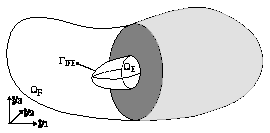
\includegraphics[scale=2.0,trim=0cm 0cm 0cm 0.0cm, clip=true]{Imagens/Cap7/dominioIFE.pdf}	
	\label{fig:dominioIFE}
	\legend{Fonte: Elaborada pela autora}
\end{figure}

O domínio computacional não se sobrepõe, por isso, é necessário que em $\boundaryFSI$ existam condições físicas adicionais para se realizar o acoplamento. \citeonline{richter2017fluid} cita que o acoplamento é garantido ao se atender as seguintes condições no contorno $\boundaryFSI$ : condição cinemática, condição dinâmica e condição geométrica.

A condição cinemática refere-se ao fato de que a velocidade do fluido e do sólido na interface devem ser iguais. A condição dinâmica, refere-se à existência de continuidade do vetor tensão de Cauchy na direção normal ao contorno $\boundaryFSI$, enquanto a condição geométrica refere-se à conformidade entre estrutura e fluido na interface.

Nos esquemas de acoplamento monolítico, as condições cinemática e dinâmica são atendidas de maneira implícita, visto que os meios são tratados no mesmo contexto matemático. Para esquemas particionadas, como o deste estudo, essas condições são atendidas através da transferência de condições de contorno apropriadas de um meio para outro durante o processo iterativo de solução, ou a cada passo de tempo.

Para a condição cinemática tem-se:

\begin{align}
	\velocity = \solidVel \ \textrm{no contorno} \ \boundaryFSI,
\end{align}

\noindent atendida através da aplicação dos valores de $\solidVel$ nos nós (ou pontos de controle) que compõe a malha do fluido na interface fluido-estrutura.

A condição dinâmica, prescreve a continuidade da tensão (da componente normal à interface para o caso de condição de parede lisa, ou de todas as componentes para o caso de condição de aderência). Neste trabalho considera-se apenas a condição de aderência, de modo que a condição dinâmica é dada por:

\begin{align}
	\stressTensorS \snormalS + \stressTensorF \snormalF = \vzero \ \textrm{no contorno} \ \boundaryFSI,
\end{align}

\noindent na qual, $\stressTensorS$ representa as tensões de Cauchy da estrutura, $\stressTensorF$ as tensões de Cauchy no fluido, e $\snormalS$ e $\snormalF$ representam os vetores normais no contorno $\boundaryFSI$ apontando para o fluido e para a estrutura,  respectivamente. Essa condição é imposta ao longo do processo bloco-iterativo de solução através da aplicação da força de superfície $\stressTensorF \snormalS$ no contorno da estrutura em contato com o fluido.

Já a condição geométrica está relacionada ao fato que os domínios computacionais $\domainS$ da estrutura e $\domainF$ do fluido devem sempre coincidir em $\boundaryFSI$, ou seja, não devem existir superposições ou frestas nessa interface. No contexto desse estudo essa condição é atendida através de uma movimentação adequada da malha local (Método Arlequin), que se deforma para acomodar a mudança de configuração da estrutura. A técnica de movimentação de malha adotada é apresentada na \autoref{capitulo:Cap7:CondAcop:MovMalha}.

\subsection{Movimentação da Malha} \label{capitulo:Cap7:CondAcop:MovMalha}

Para a satisfação da condição geométrica nos problemas de IFE desse trabalho, uma técnica adequada de movimentação de malha deve ser aplicada. É necessário que o método de movimentação de malha seja robusto o suficiente para que garanta uma discretização adequada (ou seja, com elementos geometricamente aceitáveis, com áreas e volumes maiores do que zero e com ângulos que não estejam próximos de $0^o$ nem de $180^o$) durante toda a análise.

Dentre as técnicas constantes na literatura, destacam-se aquelas que impõem os deslocamentos da estrutura na malha do fluido ao longo do contorno $\boundaryFSI$, determinando o campo de deslocamentos no restante da malha do fluido por meio da resolução de um problema de valor de contorno (PVC). Neste trabalho, será adotada essa abordagem, formulando o problema com base na equivalência entre a movimentação da malha e um problema de elasticidade linear, atribuindo-se a cada elemento uma rigidez diferente de acordo com a técnica MJBS  (\textit{Mesh-Jacobian Based Stiffening}), apresentada por  \citeonline{TezduyarBSJ:1992f} e \citeonline{TezduyarABJ:1993}, que visa preservar os aspectos dos elementos menores, impedindo inversão de elementos ou que elementos assumam volume muito pequeno.

Nesse método, o movimento da malha é determinado usando um problema da elasticidade de Dirichlet fictício, descrito como:

\begin{align}
	\int_{\domaintt} \straintensor \left(\testfunction\right) : \stressTensorM \left(\dispMh - \dispMtth \right) \deriv \domain = 0,
	\label{eq:elasticity}
\end{align}

\noindent na qual $\testfunction$ é a função teste; $\dispMh$ é o deslocamento medido da configuração de referência, com coordenadas $\posALEh$, até a configuração atual $\posh$ ($\posh = \posALEh +\dispMh $); e 
$\dispMtth$ representa o deslocamento da configuração de referência até a configuração da malha no instante ${\tildet}$, de modo que $\postth$ ($\postth = \posALE + \dispMtth$); $\stressTensorM$ representa o tensor de tensões segundo a hipótese de pequenos deslocamentos.

A escolha para $\tildet$ é geralmente $\tildet = {t_{n}}$ quando se calcula a configuração da malha no instante ${t_{n+1}}$ (ver \citeonline{Tononetal:2021} para maiores detalhes). 

O tensor de tensão é calculado através da seguinte relação:

\begin{align}
	\stressTensorM(\dispM)
	&=
	\frac{\elasticityM}{1+\poissonm}
	\left(
	\frac{\poissonm}{(1 - 2 \poissonm)}
	\trace\left(\straintensor(\dispM)\right)\unittensor
	+
	\straintensor(\dispM)
	\right)
\end{align}

\noindent com $\elasticityM$ e $\poissonm$ 	sendo respectivamente o módulo de Elasticidade e o coeficiente de Poisson fictícios. 

Nos problemas de IFE, demanda-se maior controle da resolução da malha próxima a interface dos meios fluidos e sólidos, para representar os efeitos de camada limite, e como consequência, a obtenção de soluções mais acuradas nessas regiões críticas. Por outro lado, a discretização mais refinada é mais afetada pela deformação. Assim, visando preservar a geometria dos elementos menores, deve-se aumentar para enrijecendo os menores mais do que os maiores, no método MJBS a equação da elasticidade fica descrita ao final como:

\begin{align}
	\int_{\domaintt} \straintensor \left(\testfunction\right) : \stressTensorM \left(\dispMh- \dispMtth\right) \left(\frac{\jacM}{\left({\jacM}\right)_0}\right)^{-\chi_M} \deriv \domain = 0, 
	\label{eq:elasticityMJBS}
\end{align}

\noindent onde $\jacM$ é o determinante Jacobiano do mapeamento do espaço local adimensional para a configuração do elemento em $\tilde{t}$
\begin{align}
	\jacM = det\left(\frac{\partial\postth}{\partial\adimensionalcoordinates}\right),
\end{align} 
$(\jacM)_0$ é um parâmetro livre tal que $(\jacM)_0>$, que pode ser adotado como o jacobiano médio na malha inicial, e $\chi_M$ determina a ordem pela qual a rigidez aumenta à medida que o tamanho dos elementos diminui, sendo adotado nas simulações deste trabalho $\chi_M=1,0$. 



\section{Transferência de condições de acoplamento entre as discretizações}

Em diversas situações é interessante que mas malhas do fluido e da estrutura possam ser diferentes no contorno $\boundaryFSI$, inclusive que podendo ter aproximações distintas. Assim, é importante uma metodologia que possibilita o acoplamento de discretizações com nós não coincidentes na interface fluido-estrutura. 

O procedimento adotado nesse trabalho pode ser entendido a partir da \autoref{fig:contornoIFE}. Durante a etapa de pré-processamento, cada nó do contorno da estrutura $\ePosition_E$ é projetado sobre o contorno do fluido, indentificando-se a coordenada local do ponto do fluido  mais próximo $\adimensionalcoordinates_F (\ePosition_E)$, bem como o elemento em que está inserido. Da mesma forma, cada nó do contorno do fluido $\pos_F$ é projetado sobre o contorno da estrutura, e encontra-se uma coordenada paramétrica equivalente $\adimensionalcoordinates_E(\pos_F)$. 

\textcolor{red}{A forma mais correta de fazer é projetar cada ponto de quadratura da estrutura no fluido para poder calcular a força de superfície. Isso está explicado no artigo do Jeferson de 2019. Na forma como você está apresentando (acredito que seja também o que está implementado), as forças de superfície vão ser aproximadas pelas funções de forma do sólido.... (Veja seção 4.1-4.3 do artigo do Jeferson)}


\textcolor{red}{Está faltando explicar a transferência das condições de acoplamento (seção 4.3 do artigo do Jeferson)}


\begin{figure}[!htbp]
	\caption{Discretizações não-coincidentes no contorno IFE}
	\centering 
	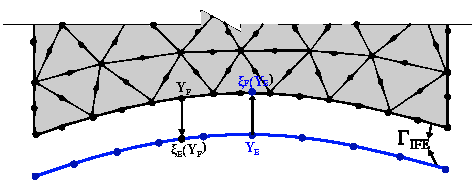
\includegraphics[scale=1.5,trim=0cm 0cm 0cm 0cm, clip=true]{Imagens/Cap7/contornoIFE.pdf}	
	\label{fig:contornoIFE}
	\legend{Fonte: Elaborada pela autora}

\textcolor{red}{A figura não parece mostrar os pontos mais próximos (projeção normal ao contorno), mas sim uma projeção vertical, isso porque você afastou artificialmente os contornos... Não precisa mudar, mas é bom registrar isso. Os símbolos também estão diferentes do texto.}
\end{figure}

De maneira prática, para cada nó do fluido, é aplicada a velocidade interpolada na malha da estrutura sobre as coordenadas locais referentes ao nó do fluido. O mesmo é feito para o deslocamento da malha do fluido. Já para a estrutura, em cada nó, calcula-se .... \parei aqui....
em cada uma das coordenadas locais relativas a cada nó na malha de fluido, e após isso aplicadas a este nó. O equivalente ocorre quando os dados são provenientes do fluido e serão transmitidos a estrutura.

\section{Acoplamento Particionado Forte - Bloco-Iterativo}

Os problemas de IFE são caracterizados pela interdependência entre o fluido e a estrutura, visto que o comportamento do escoamento depende do formato e do movimento da estrutura, enquanto que o movimento da estrutura e sua deformação dependem das forças do fluido que atuam sobre ela. Matematicamente pode-se dizer que os problemas de IFE são conjuntos de equações e condições de contorno associadas ao fluido e a estrutura que devem ser satisfeitas simultaneamente.

As equações completas discretizadas da formulação IFE conduzem a um sistema de equações não-lineares que devem ser resolvidas a cada passo de tempo e podem ser representadas da seguinte maneira \cite{BazilevsTT:2013}:

\begin{align}
	\Nf\left(\df,\ds,\dm\right) = \vzero, \label{eq:N1}\\ 
	\Ns\left(\df,\ds,\dm\right) = \vzero,\label{eq:N2}\\
	\Nm\left(\df,\ds,\dm\right) = \vzero \label{eq:N3},
\end{align}

\noindent em que $\Nf$, $\Ns$ e $\Nm$ representam as equações que descrevem o fluido, a estrutura e a malha respectivamente, e, $\df$, $\ds$, $\dm$ são vetores com as variáveis nodais de cada meio. 
A resolução dessas equações através do método de Newton-Raphson conduz ao seguinte sistema linear de equações:

\begin{align}
	\begin{bmatrix}
		\mA_{11} & \mA_{12} & \mA_{13} \\
		\mA_{21} & \mA_{22} & \mA_{23} \\
		\mA_{31} & \mA_{32} & \mA_{33}
	\end{bmatrix}
	\begin{bmatrix}
		\xf \\
		\xs \\
		\xm
	\end{bmatrix}
	&=
	\begin{bmatrix}
		\cff \\
		\css \\
		\cmm
	\end{bmatrix}.
	\label{eq:sist_lin_IFE}
\end{align}	

\noindent sendo $\cff = - \Nf$, $\css = - \Ns$, $\cmm = - \Nm$. $\xf$, $\xs$ e $\xm$ são os incrementos às soluções $\df$, $\ds$ e $\dm$ respectivamente e $\mA_{ij} = \frac{\partial\Ni}{\partial\djj}$. 

 \citeonline{BazilevsTT:2013} apresentam uma classificação da metodologia de acoplamento segundo a forma de resolver essas equações não-lineares. As categorias definidas pelos autores são: técnica direta, técnica bloco-iterativa e técnica quase-direta. 

A técnica direta seria equivalente aos esquemas de solução monolíticos citados ao longo do texto, e consiste na resolução a cada iteração de Newton-Raphson do sistema apresentado na \autoref{eq:sist_lin_IFE}. Essa técnica apresenta boa convergência, entretanto, devido aos grandes sistemas lineares gerados, ocorre um aumento do custo computacional.

Nesse contexto, e buscando proporcionar um total desacoplamento entre os \textit{solvers} de fluido e de estrutura, adotou-se o um esquema de acoplamento do tipo particionado forte. Dentro da classificação dos autores \citeonline{BazilevsTT:2013} seria equivalente a técnica de acoplamento do tipo bloco iterativo.

Quando se utiliza um acoplamento do tipo bloco iterativo, os sistemas do fluido, da estrutura e da malha são tratados em blocos separados, e para cada iteração dentro de um passo de tempo, se resolve sequencialmente o seguinte conjunto de equações:

\begin{align}
	\left .\frac{\partial\Nf}{\partial\df}\right|_{\left(\df^{i},\ds^{i},\dm^{i}\right)} \Delta\df^{i} = - \Nf\left(\df^{i},\ds^{i},\dm^{i}\right)  \label{eq:lin_fluido} \\
	\df^{i+1} =  \df^{i} + \Delta\df^{i} \label{eq:atu_fluido}	\\
	\left.\frac{\partial\Ns}{\partial\ds}\right|_{\left(\df^{i+1},\ds^{i},\dm^{i}\right)} \Delta\ds^{i} = - \Ns\left(\df^{i+1},\ds^{i},\dm^{i}\right) \label{eq:lin_est}\\
	\ds^{i+1} =  \ds^{i} + \Delta\ds^{i} \label{eq:atu_est}\\
	\left.\frac{\partial\Nm}{\partial\dm}\right|_{\left(\df^{i+1},\ds^{i+1},\dm^{i}\right)} \Delta\dm^{i} = - \Nm\left(\df^{i+1},\ds^{i+1},\dm^{i}\right) \label{eq:lin_malha}\\
	\dm^{i+1} =  \dm^{i} + \Delta\dm^{i}  \label{eq:atu_malha}
\end{align}

Nota-se que o ocorre é apenas uma modificação da matriz tangente com relação ao método direto. Este fato, faz com que a resposta não seja alterada, entretanto, a convergência do problema pode ser afetada. 

Em certos problemas envolvendo estruturas leves, a resposta estrutural pode tornar-se extremamente sensível a pequenas variações nas forças provenientes do fluido. Esse fenômeno pode levar à divergência da técnica de bloco iterativo. Para contornar essa dificuldade, adotou-se a estratégia proposta por \citeonline{Tezduyar:2003d}, chamada de \textit{Augmented A22} na qual a matriz de massa em $\mA_{22}$ é aumentada por um fator dependente do tipo de problema em análise. Essa modificação ocorre sem alterar $\cff$, $\css$ e $\cmm$, ou seja, sem modificar as equações não lineares. Dessa forma, quando a solução pelo método de bloco iterativo converge, a massa estrutural real do problema permanece inalterada.

\subsection{Implementação Computacional} 

O Algoritmo que descreve a implementação computacional do problema de IFE de acordo com a técnica de acoplamento forte do tipo bloco-iterativo é apresentada no Alg. \ref{alg:IFE}.

\begin{algorithm}
	\caption{Algoritmo para solução de problemas IFE}
	\label{alg:IFE}
	\begin{algorithmic}[1]
		\State Busca por coordenadas paramétricas correspondentes aos nós da malha do fluido na malha da estrutura;
		\State Busca por coordenadas paramétricas correspondentes aos nós da malha da estrutura na malha do fluido;
		\For {o passo de tempo $t=0$ até $t=\totalTime$} 
		\State Atualiza as variáveis do fluido, estrutura e malha no passo de tempo $t = t-1$;
		\For {número de iterações de Newton Raphson $it=0$ até $it=N_{it}$}
		\State \textbf{Fluido}
		\State Realiza os passos das linhas 1., 2., 3. e 4. do Algoritmo \ref{alg:fluidARLQ};
		\State Resolve o problema do fluido (\autoref{eq:lin_fluido});
		\State Atualiza as variáveis do fluido na iteração $it$ através da \autoref{eq:atu_fluido};
		\State Calcula medida de convergência $\epsilon_F$;
		\State Atualiza as forças de superfície no contorno  $\boundaryFSI$ ($\boldsymbol{t^{E}} = -\stressTensorF \cdot \snormalF$) ;
		\State \textbf{Estrutura}
		\State Resolve o problema da estrutura (\autoref{eq:lin_est});
		\State Atualiza as variáveis da estrutura na iteração $it$ através da \autoref{eq:atu_est};
		\State Calcula medida de convergência $\epsilon_E$;
		\State Atualiza velocidade e acelerações no fluido no contorno  $\boundaryFSI$;
		\State Atualiza posição da interface da malha no contorno  $\boundaryFSI$;
		\State \textbf{Malha}
		\State Resolve o problema de malha através da \autoref{eq:lin_malha};
		\State Atualiza as variáveis da malha na iteração $it$ através da \autoref{eq:atu_malha};
		\State Calcula medida de convergência $\epsilon_M$;
		\If    {$\epsilon_F$, $\epsilon_E$ e $\epsilon_M$ < $tol$ } 
		\State Sair do loop;
		\EndIf
		\EndFor
		\EndFor
	\end{algorithmic}
\end{algorithm}

No algoritmo apresentado $\boldsymbol{t^{E}}$ representa as forças de superfície no contorno $\boundaryFSI$ aplicadas à estrutura, e as medidas de convergência $\epsilon_F$, $\epsilon_E$ e $\epsilon_M$ são normas vetoriais $L_2$ aplicadas sobre o resíduo das respectivas equações diferenciais.

\section{Exemplos}

Para a validação da metodologia de análise de problemas de IFE, apresentada nesse capítulo, alguns exemplos serão estudados e analisados.

Os dois primeiros exemplos dizem respeito a uma cavidade com um fundo flexível composto por uma chapa, com velocidade oscilatória aplicada em seu topo. Esses exemplos são uma extensão do típico problema da DFC de uma cavidade quadrada (apresentado, por exemplo, na \autoref{capitulo:Cap2:VerApl:CavQuad}) e serão apresentados em uma versão bidimensional e tridimensional.

O seguinte exemplo consiste em um painel flexível engastado a um bloco prismático rígido. Esse problema é comumente utilizado na validação de códigos de Interação Fluido-Estrutura (IFE), pois envolve fenômenos complexos. À medida que ocorre o desprendimento de vórtices devido ao escoamento ao redor do prisma, perturbações são geradas no fluxo, excitando a estrutura, que então sofre grandes deslocamentos.

\subsection{Cavidade com fundo flexível - 2D}

O problema da cavidade com fundo flexível trata-se de uma extensão do típico problema da DFC de uma cavidade quadrada com velocidade prescrita em sua parede superior. Sua simulação computacional já foi realizada por diversos autores, como por exemplo, \citeonline{GerbeauV:2003} e \citeonline{Yokomizo:2024}, e  por isso, será utilizada no processo de validação da metodologia nesta tese apresentada.

A cavidade com fundo flexível (geometria apresentada na \autoref{fig:cavFF2d_geometria}) consiste em uma cavidade composta por paredes laterais rígidas e um fundo flexível composto por uma placa fina de 0,002. No seu topo uma velocidade oscilatória horizontal $u_1(t)=1-cos(0,4 \pi t)$ é aplicada, sendo as demais velocidades ($u_2$ e $u_3$) nessa parede nulas. Condições de contorno de não deslizamento são aplicadas as paredes laterais. Esse modelo de cavidade apresenta duas aberturas de 0,1 no topo de suas laterais com condições homogêneas de Neumann. O problema apresenta comportamento bidimensional, e por isso será analisado utilizando-se uma discretização 3D com uma espessura de 0,1 de profundidade. Adotou-se condição de simetria para o fluido na direção $y_3$.  Na \autoref{fig:cavFF2d_geometria} são apresentadas também as propriedades físicas do fluido e da estrutura necessárias a análise.

\begin{figure}[!htbp]
	\caption{Cavidade fundo flexível 2D: geometria}
	\centering 
	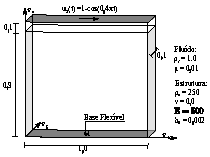
\includegraphics[scale=2.5,trim=0cm 0cm 0cm 0cm, clip=true]{Imagens/Cap7/cavFF2d_geometria.pdf}	
	\label{fig:cavFF2d_geometria}
	\legend{Fonte: Elaborada pela autora}
\end{figure}

A placa fina possui condições de deslocamentos nulos em suas laterais esquerda e direita, e, na direção perpendicular ao plano da cavidade o vetor generalizado e os deslocamentos, nesta direção, são prescritos como zero em $y_3=0,0$ e $y_3=0,1$.

No que diz respeito a integração temporal utilizou-se $\timeStep = 0,1$, e $\specRadius = 0,0$. A escolha por uma integração temporal com máxima dissipação se deu por conta do trabalho de \citeonline{Forsteretal:2007} que reporta que a regra trapezoidal de integração leva a resultados instáveis para esse problema.

Foram utilizadas nas análises três diferentes discretizações para o modelo Arlequin, sendo as malhas globais em discretização isogeométrica com funções de forma quadráticas (IGA) e as malhas locais, mais refinadas e estruturadas, em elementos finitos (MEF) tetraédricos quadráticos. Além disso, os resultados foram comparados com uma discretização somente em elementos finitos tetraédricos quadráticos, chamada de monomodelo. A quantidade de nós, ou pontos de controle (PC), e de elementos ou células, para cada uma dessas discretizações é apresentada na \autoref{tab:CF2DD}, assim como detalhes da discretização da placa, na qual foram utilizados elementos triangulares quadráticos estruturados. Na tabela ML e MG são abreviações para malha local e malha global respectivamente, e El representa os elementos ou células.
	
	\begin{center}
		\begin{table}[!htbp]
			\caption{Cavidade fundo flexível 2D: Discretizações}
			\centering
			\begin{tabular}{ccccc} 
				\toprule
				\ &  Nós/PC-ML & El-ML & Nós/PC-MG & El-MG  \\ 
				\midrule \midrule
				Arlequin - Malha 0 & 315 & 120 & 504 & 100 \\ 
				\midrule
				Arlequin - Malha 1 & 1107 & 480 & 1584 & 400\\
				\midrule
				Arlequin - Malha 2 & 4131 & 1920 & 5544 & 1600\\
				\midrule
				Monomodelo & - & - & 9389 & 4563\\
				\midrule
				Estrutura - Malha 0 & - & - &  63 & 20\\
				\midrule
				Estrutura - Malha 1 & - & - &  123 & 40\\
				\midrule
				Estrutura - Malha 2 & - & - &  243 & 80 \\
				\midrule
			\end{tabular}
			\label{tab:CF2DD}
			\fonte{Elaborada pelos autores.}%
		\end{table}
	\end{center}

A malha isogeométrica utilizada foi composta por 2 \textit{patches} (observar Figura \ref{fig:cavFF2d_malhaArlq2} para a Malha 2). Essa discretização usando 2 \textit{patches} foi necessária para gerar pontos de controle interpolatórios posicionados na linha que separa as paredes laterais das aberturas, possibilitando a adequada aplicação das condições de contorno. Na Figura \ref{fig:cavFF2d_malhaArlq2} pode ser observada também a composição do modelo Arlequin. A região em vermelho da malha local corresponde aos elementos que fazem parte da zona de colagem.  A espessura da zona de colagem foi definida como $0,1$. A constante do operador de acoplamento $L^{2}$ foi especificada como $k_{0} = 10$. A quantidade de elementos na zona de colagem para malha 0, 1 e 2  foram respectivamente de 60, 240, 960, e de nós 189, 615 e 2187. Na Figura \ref{fig:cavFF2d_malha_monomodelo} apresenta-se a malha do monomodelo e na Figura \ref{fig:cavFF2d_malha_casca} a malha 2 da casca.

\begin{figure}[!htbp]
	\caption{Cavidade fundo flexível 2D: Discretizações}
	\centering
	\subfloat[Modelo Arlequin - Malha 2\label{fig:cavFF2d_malhaArlq2}] {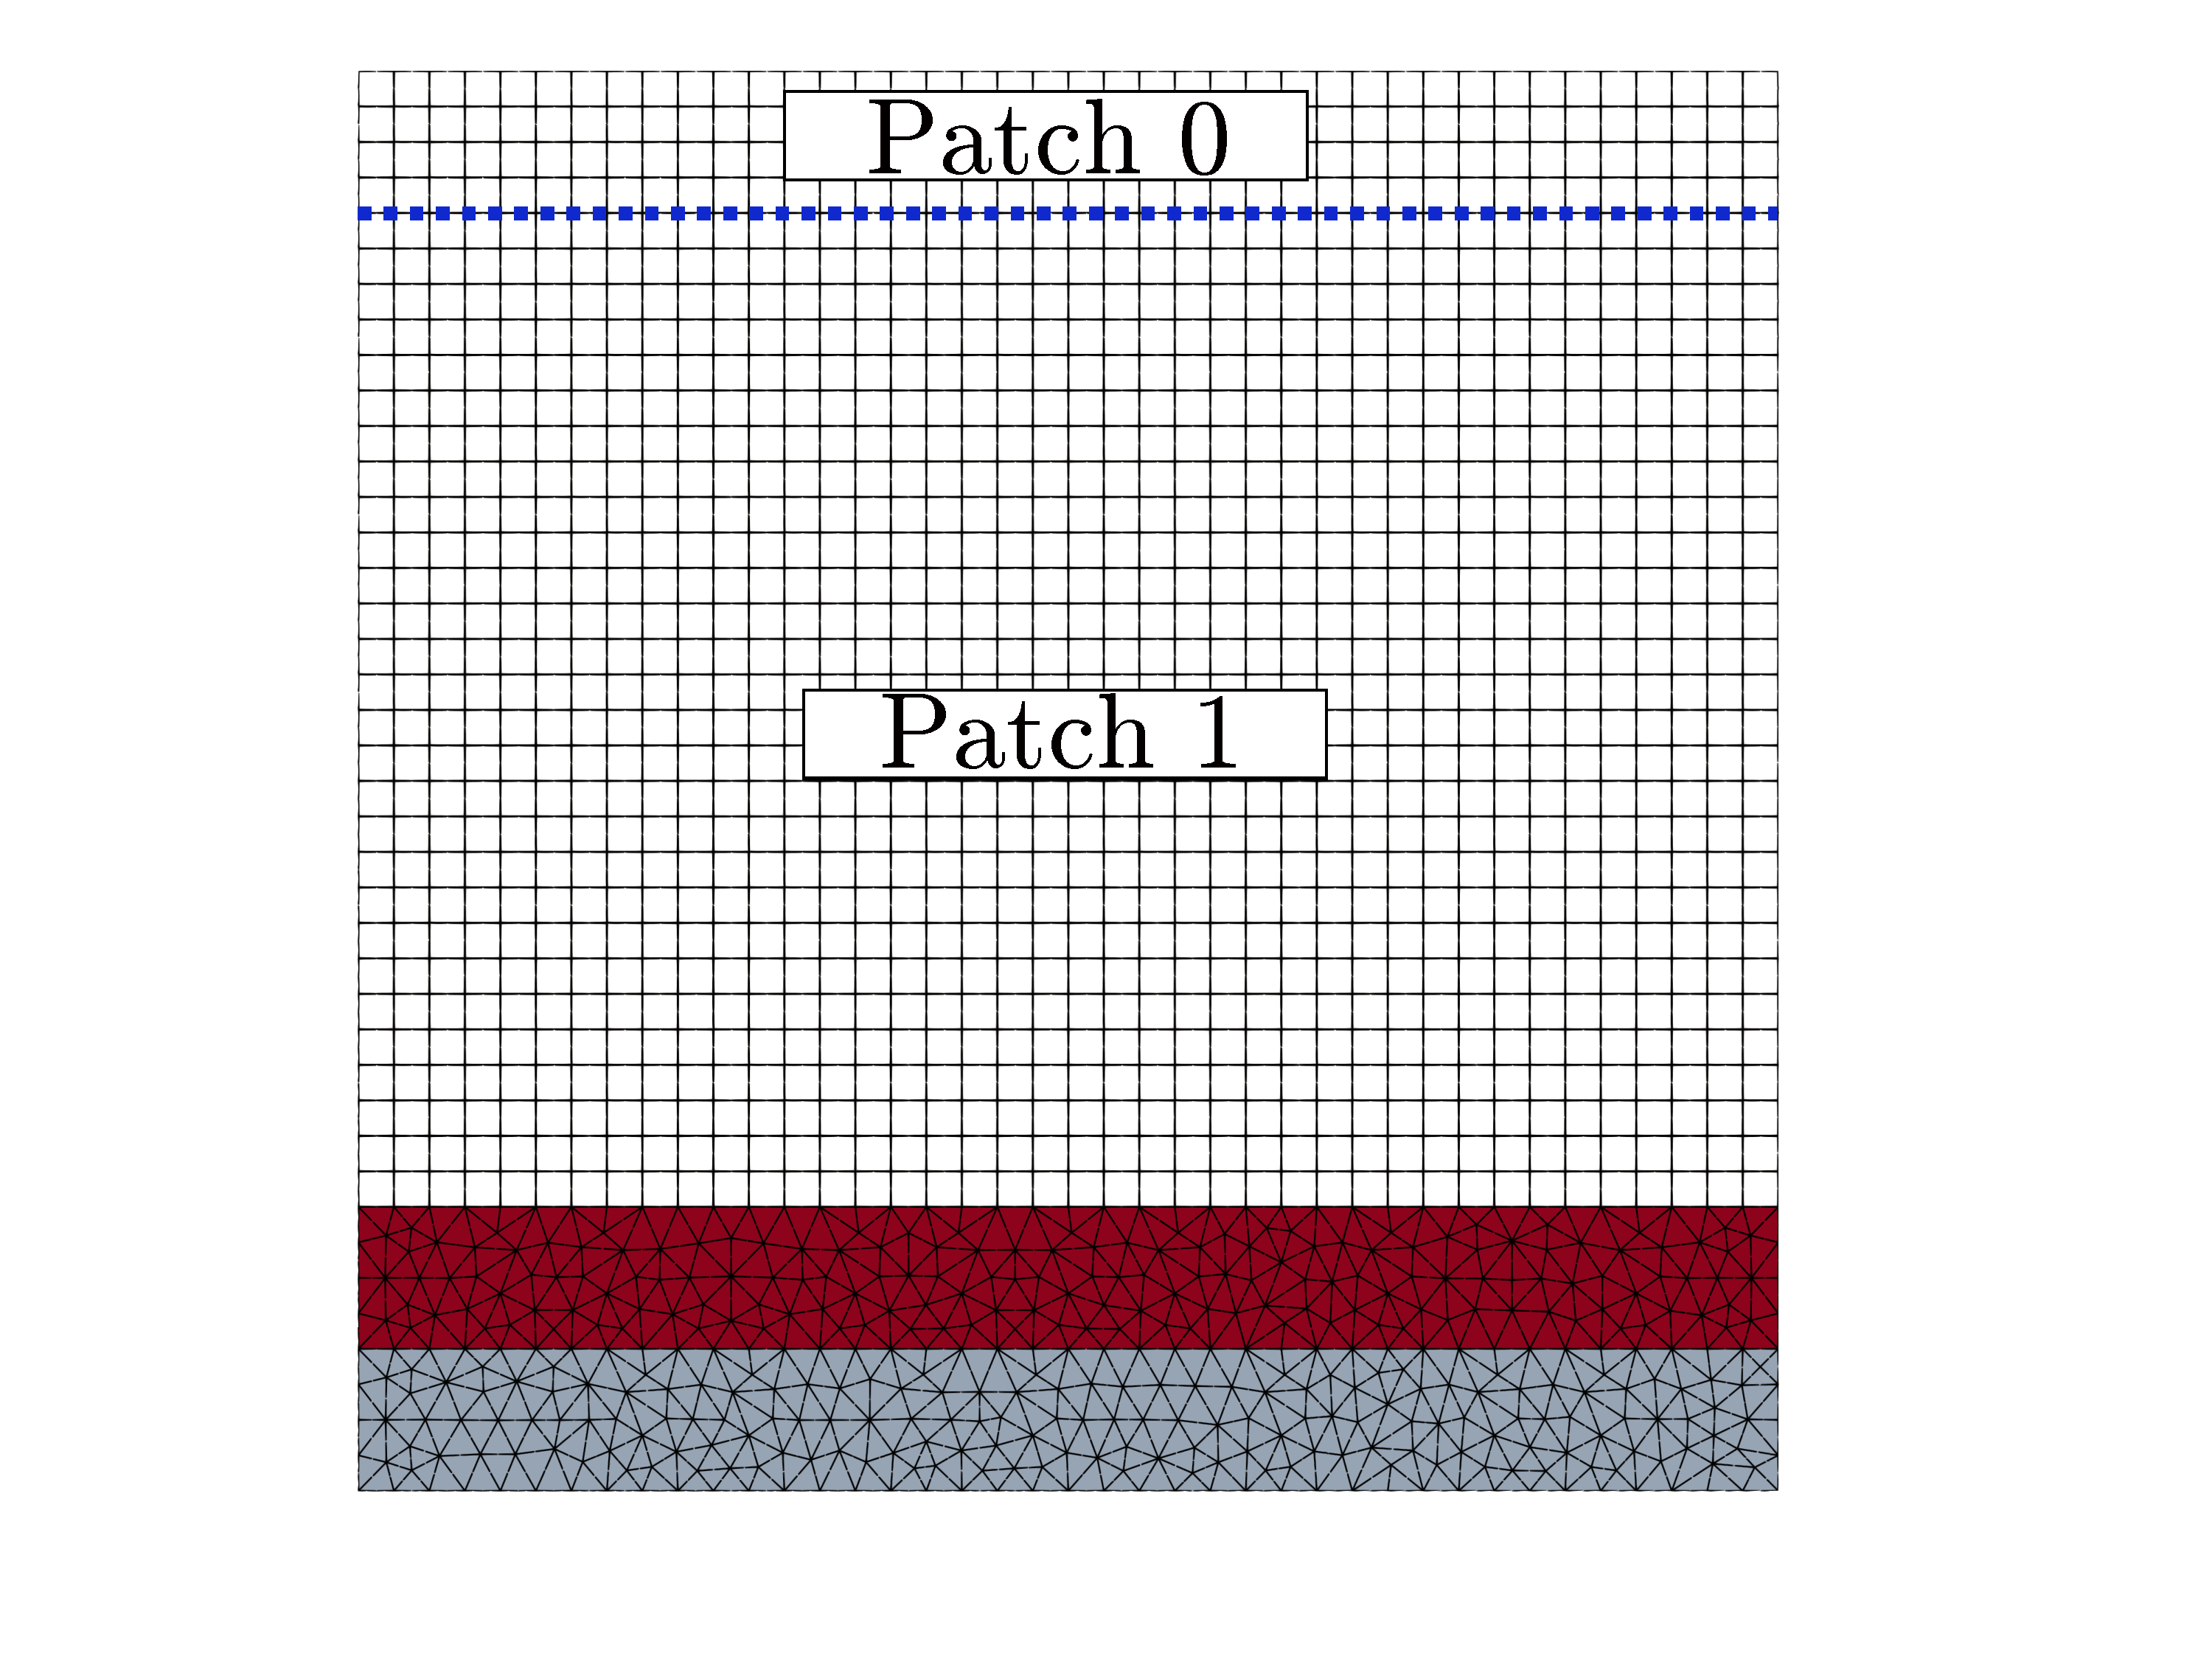
\includegraphics[scale=1.0,trim=0.5cm 0cm 0cm 0cm, clip=true]{Imagens/Cap7/cavFF2d_malha.pdf}}  \
	 \subfloat[Monomodelo\label{fig:cavFF2d_malha_monomodelo}]{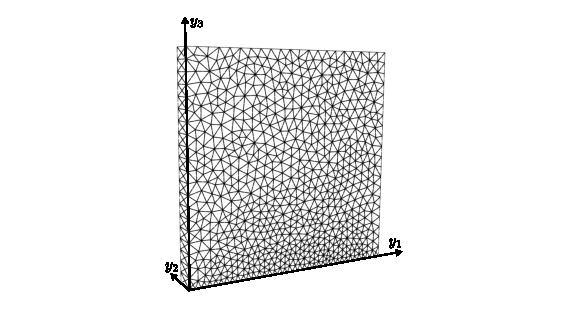
\includegraphics[scale=1.0,trim=2cm 0cm 2cm 0cm, clip=true]{Imagens/Cap7/cavFF2d_malha_mono.pdf}}  \\
	 \subfloat[Casca - Malha 2\label{fig:cavFF2d_malha_casca}]{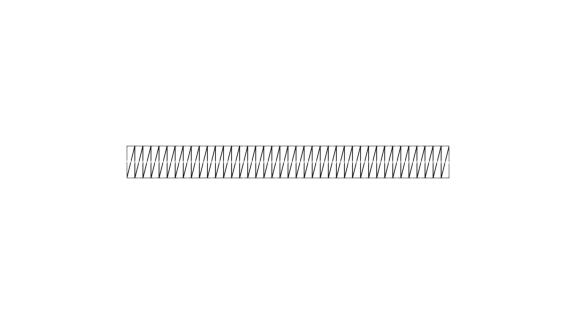
\includegraphics[scale=1.0,trim=2cm 2cm 2cm 2cm, clip=true]{Imagens/Cap7/cavFF2d_malha_casca.pdf}} 
	\label{fig:cavFF2d_malha}
	\legend{Fonte: Elaborada pela autora}
\end{figure}

Nesse problema foi necessário para atingir a convergência a utilização da técnica \textit{Augmented A22}, multiplicando-se a parcela da matriz tangente referente à matriz de massa da estrutura por um fator 2,0.

Na \autoref{fig:cavFF2d_Arlq_deslA} são apresentados os deslocamentos da placa no ponto A (ver Figura \ref{fig:cavFF2d_geometria}) para os modelos Arlequin (malha 0, malha 1 e malha 2). Para a comparação com as referências e com o monomodelo, utilizou-se o modelo Arlequin composto pela malha 2, mais refinada, e os resultados são apresentados na \autoref{fig:cavFF2d_deslA}. Pode-se observar nessa última figura, que os dados obtidos com o modelo Arlequin são compatíveis com os obtidos com o monomodelo. As diferenças encontradas entre a amplitude dos deslocamentos obtidos nesse trabalho com as referências podem ser atribuídas para as diferentes formulações e discretizações adotadas para a modelagem do fluido e da chapa. Vale ressaltar, que apesar das discretizações distintas entre o monomodelo e o modelo Arlequin, os resultados obtidos se mostraram muito satisfatórios.

\begin{figure}[!htbp]
	\caption{Cavidade fundo flexível 2D: Deslocamento em A para malhas do modelo Arlequin}
	\centering 
	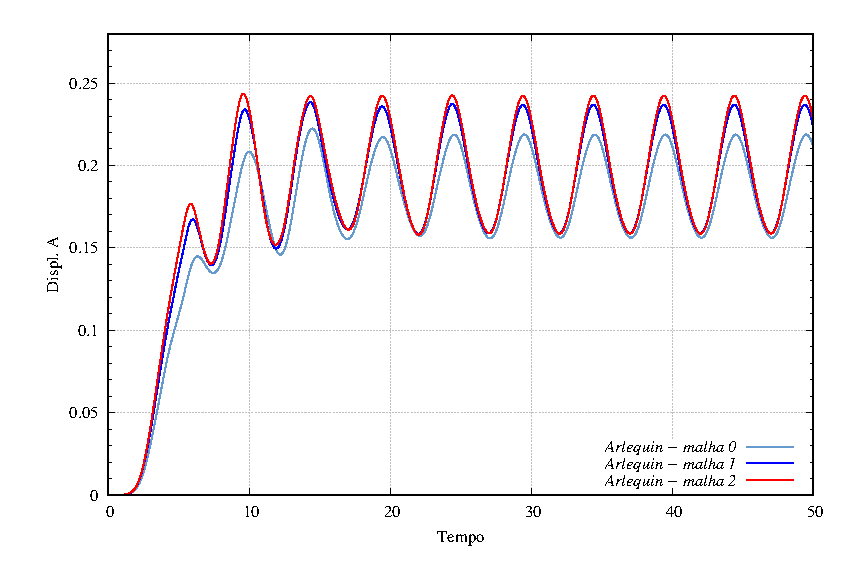
\includegraphics[scale=1.0,trim=0cm 0cm 0cm 0cm, clip=true]{Imagens/Cap7/cavFF2d_Arlq_deslA.eps}	
	\label{fig:cavFF2d_Arlq_deslA}
	\legend{Fonte: Elaborada pela autora}
\end{figure}

\begin{figure}[!htbp]
	\caption{Cavidade fundo flexível 2D: Deslocamento em A comparado com as referências e monomodelo}
	\centering 
	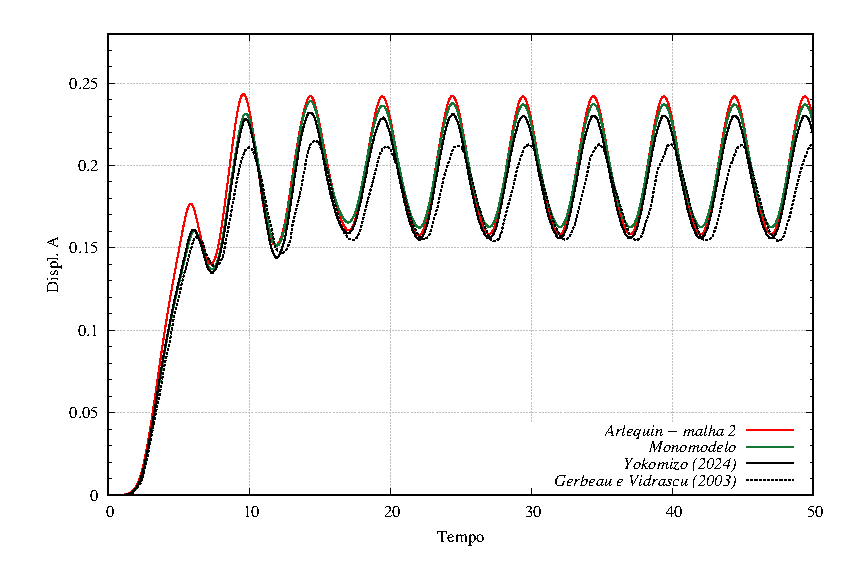
\includegraphics[scale=1.0,trim=0cm 0cm 0cm 0cm, clip=true]{Imagens/Cap7/cavFF2d_deslA.eps}	
	\label{fig:cavFF2d_deslA}
	\legend{Fonte: Elaborada pela autora}
\end{figure}

Na Figura \ref{fig:cavFF2d_vel} são apresentados os campos de velocidade em diferentes tempos da análise. Na Figura \ref{fig:cavFF2d_press} são apresentados os campos de pressão nesses mesmos tempos de análise.

\begin{figure}[!htbp]
	\caption{Cavidade fundo flexível 2D: Campos de velocidade}
	\centering
	\subfloat[$t = 4,0 $]{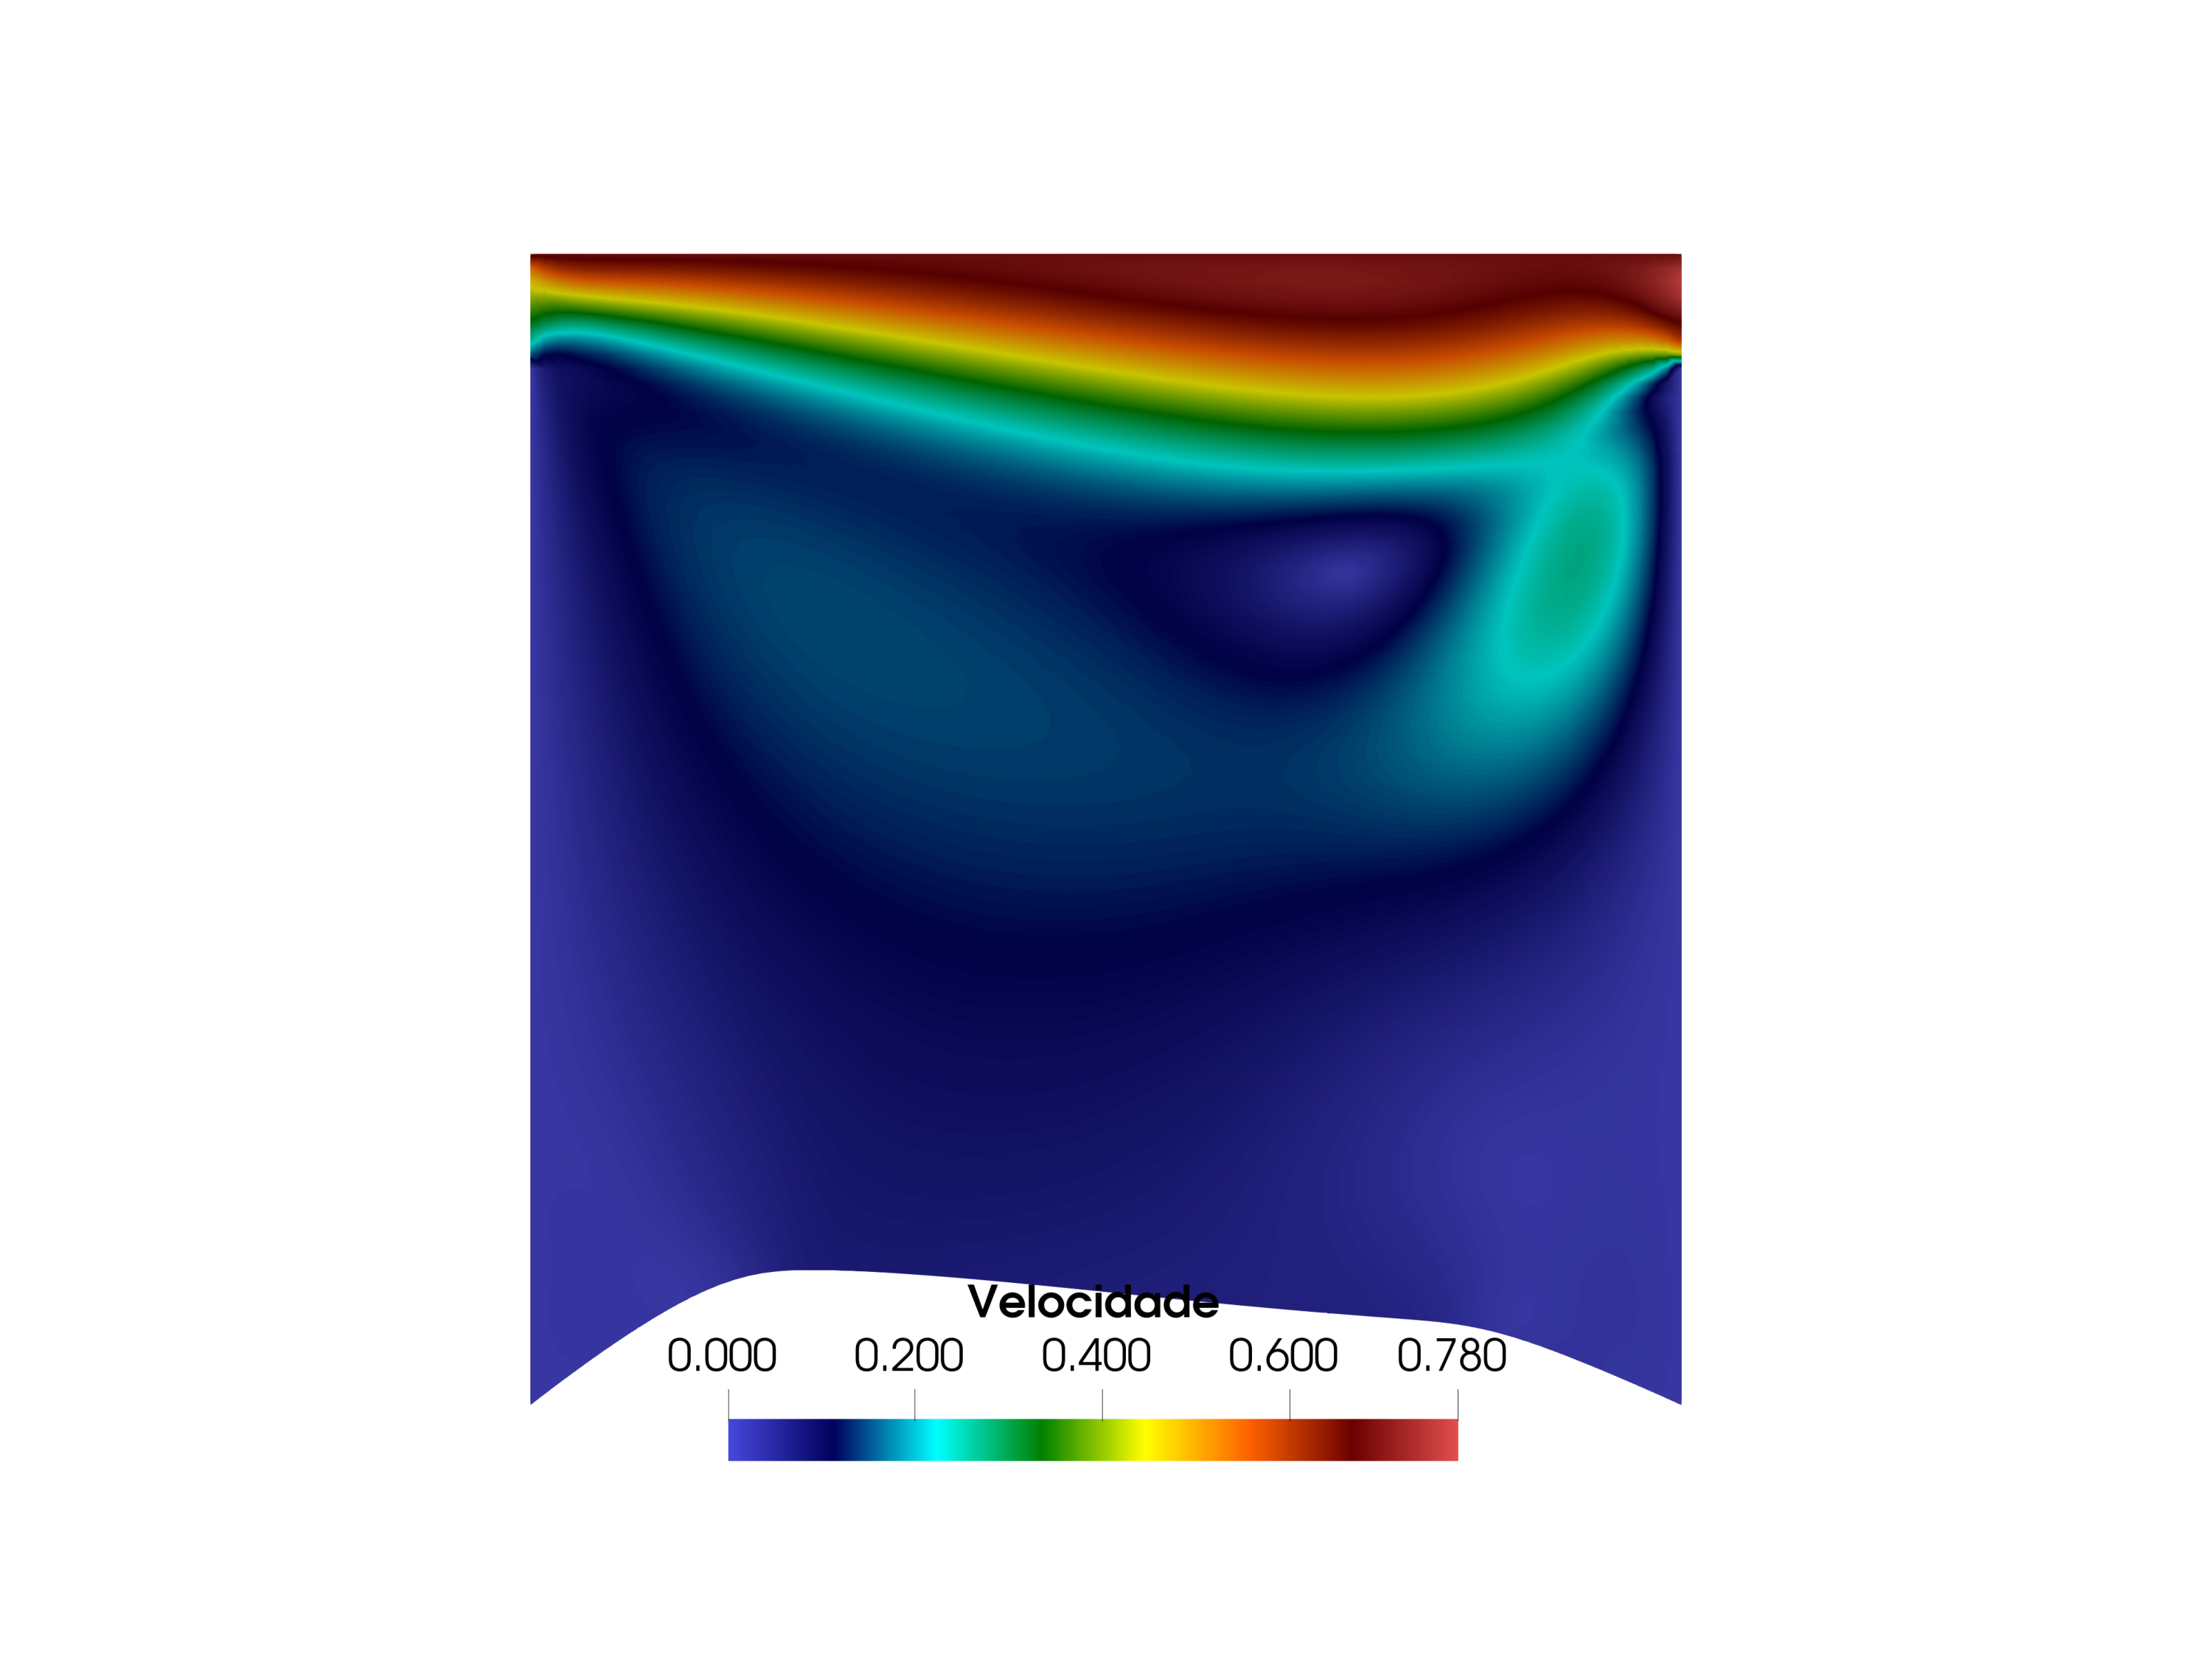
\includegraphics[scale=1.2,trim=2cm 0cm 2cm 1cm, clip=true]{Imagens/Cap7/cavFF2d_vel4.pdf}} \
	\subfloat[$t = 8,0 $]{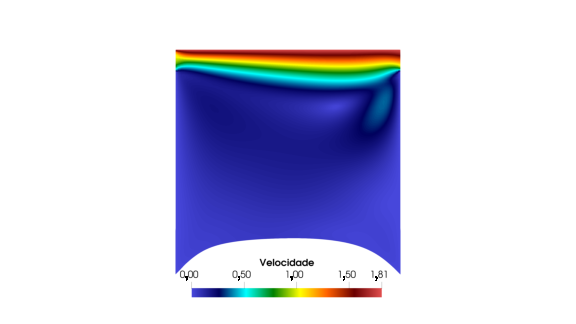
\includegraphics[scale=1.2,trim=2cm 0cm 2cm 1cm, clip=true]{Imagens/Cap7/cavFF2d_vel8.pdf}} \
	\subfloat[$t = 14,0 $]{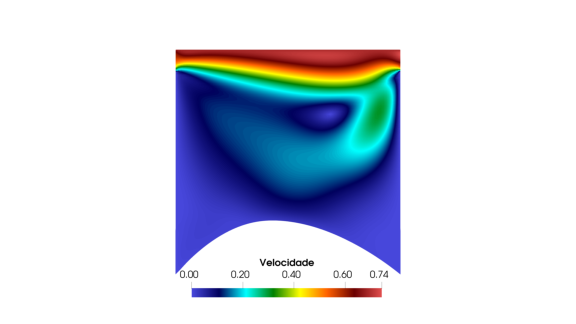
\includegraphics[scale=1.2,trim=2cm 0cm 2cm 1cm, clip=true]{Imagens/Cap7/cavFF2d_vel14.pdf}} \
	\subfloat[$t = 21,0 $]{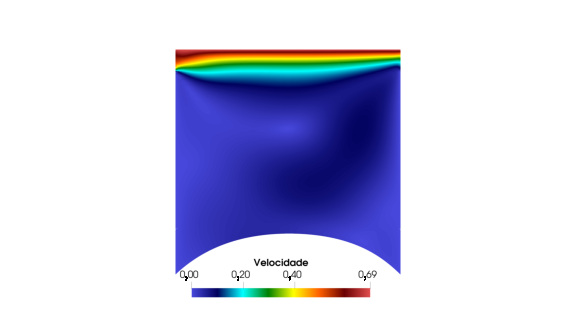
\includegraphics[scale=1.2,trim=2cm 0cm 2cm 1cm, clip=true]{Imagens/Cap7/cavFF2d_vel21.pdf}}
	\label{fig:cavFF2d_vel}
	\legend{Fonte: Elaborada pela autora}
\end{figure}

\begin{figure}[!htbp]
	\caption{Cavidade fundo flexível 2D: Campos de Pressão}
	\centering
	\subfloat[$t = 4,0 $]{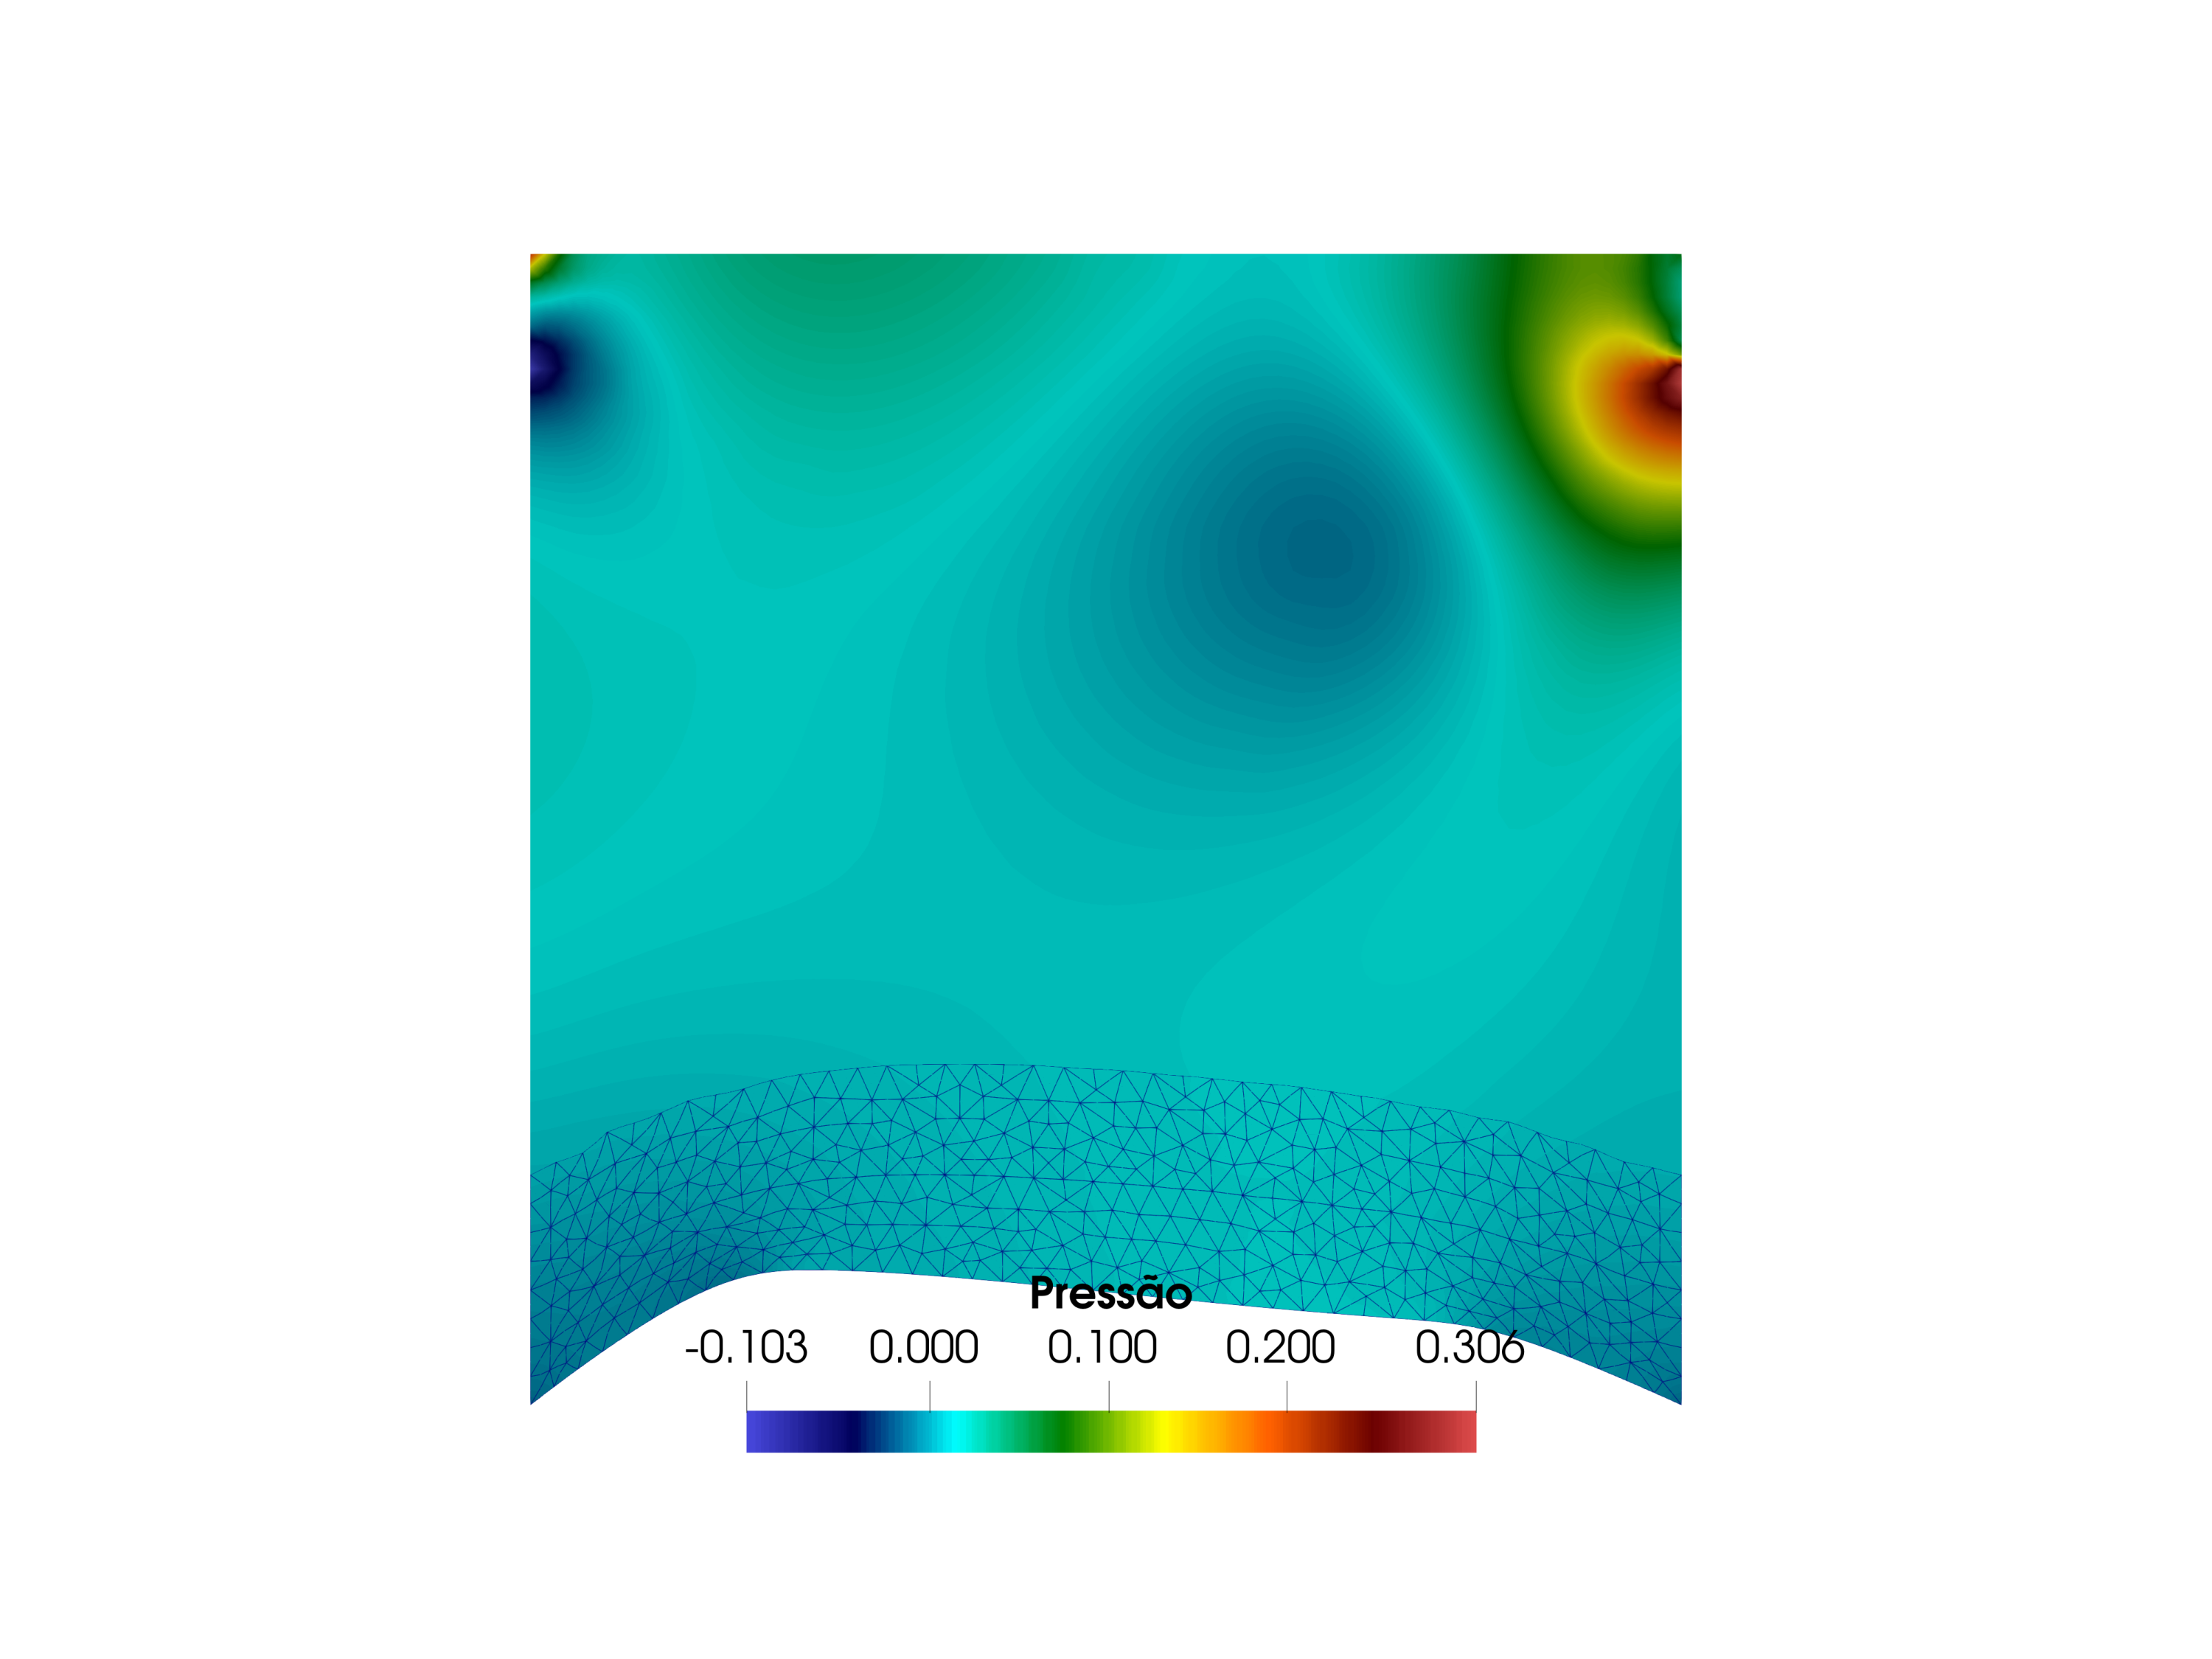
\includegraphics[scale=1.2,trim=2cm 0cm 2cm 1cm, clip=true]{Imagens/Cap7/cavFF2d_press4.pdf}} \
	\subfloat[$t = 8,0 $]{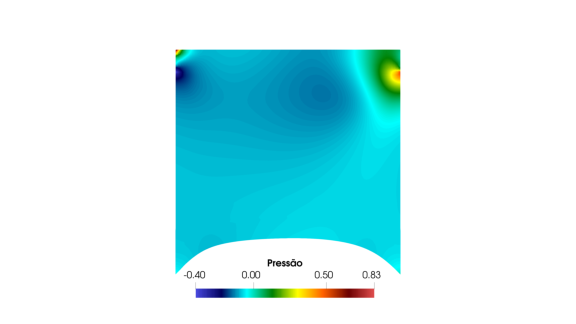
\includegraphics[scale=1.2,trim=2cm 0cm 2cm 1cm, clip=true]{Imagens/Cap7/cavFF2d_press8.pdf}} \
	\subfloat[$t = 14,0 $]{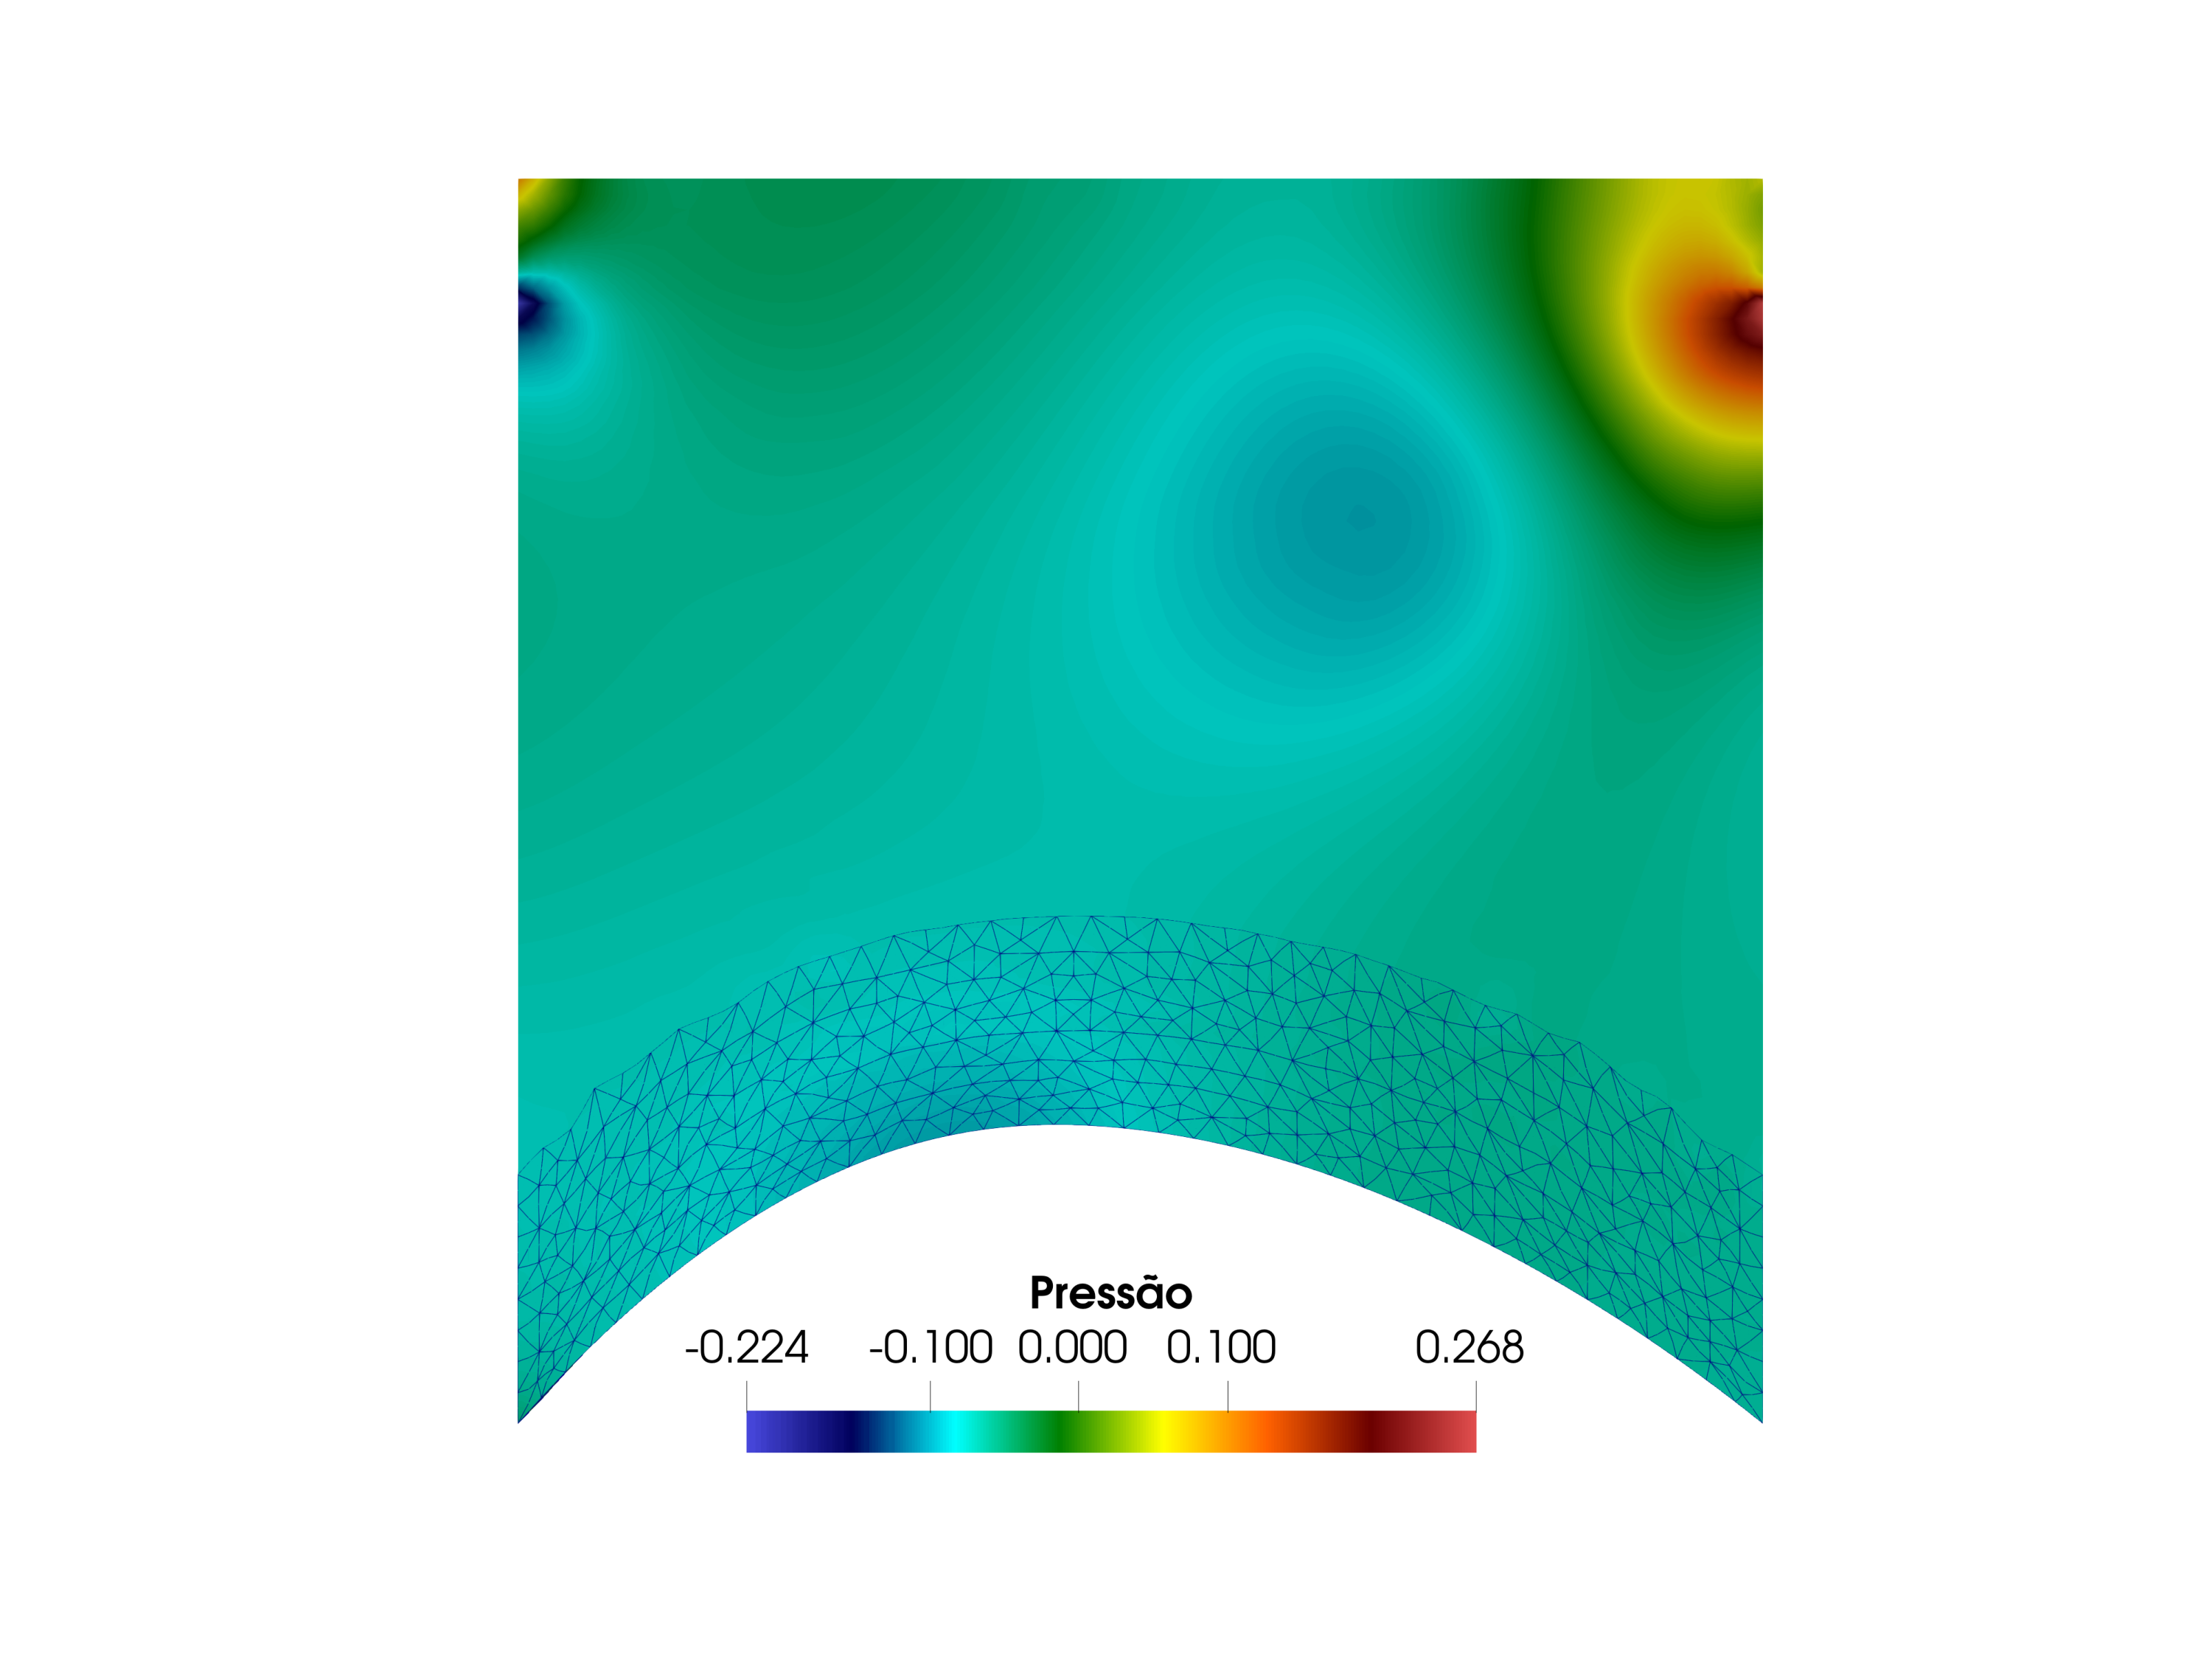
\includegraphics[scale=1.2,trim=2cm 0cm 2cm 1cm, clip=true]{Imagens/Cap7/cavFF2d_press14.pdf}} \
	\subfloat[$t = 21,0 $]{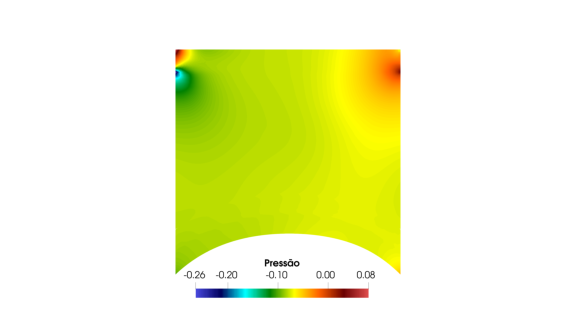
\includegraphics[scale=1.2,trim=2cm 0cm 2cm 1cm, clip=true]{Imagens/Cap7/cavFF2d_press21.pdf}}
	\label{fig:cavFF2d_press}
	\legend{Fonte: Elaborada pela autora}
\end{figure}

\subsection{Cavidade com fundo flexível - 3D}

O problema da cavidade tridimensional com fundo flexível foi proposto inicialmente por \citeonline{Mok:2001} e é muito semelhante ao 2D, entretanto, nessa variação a profundidade da cavidade possui dimensão unitária, conforme pode ser visualizado na \autoref{fig:cavFF3d_geometria}, além disso, a chapa possui restrição de deslocamentos em todos os 4 bordos. Os demais dados necessários à análise são idênticos ao do problema 2D.

\begin{figure}[!htbp]
	\caption{Cavidade fundo flexível 3D: Geometria}
	\centering 
	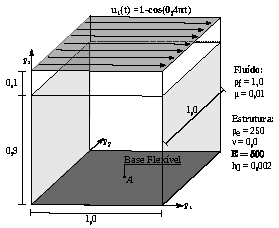
\includegraphics[scale=2.0,trim=0cm 0cm 0cm 0cm, clip=true]{Imagens/Cap7/cavFF3d_geometria.pdf}	
	\label{fig:cavFF3d_geometria}
	\legend{Fonte: Elaborada pela autora}
\end{figure}

Foram utilizadas nas análises desse problema duas diferentes discretizações: 1. Modelo Arlequin (ver Figura \ref{fig:cavFF3d_malha}), sendo a malha global em discretização isogeométrica (IGA) com funções base quadráticas e a malha local, mais refinada e estrutura, em elementos finitos (MEF) tetraédricos quadráticos; 2 . Monomodelo (Figura \ref{fig:cavFF3d_malha_mono.pdf}) discretizado com elementos finitos tetraédricos quadráticos. Para ambos modelos utilizou-se uma placa discretizada com elementos finitos triangulares quadráticos, apresentada na Figura \ref{fig:cavFF3d_malhaPlaca}.

\begin{figure}[!htbp]
	\caption{Cavidade fundo flexível 3D: Discretização}
	\centering
	\subfloat[Malhas do modelo Arlequin \label{fig:cavFF3d_malha}]{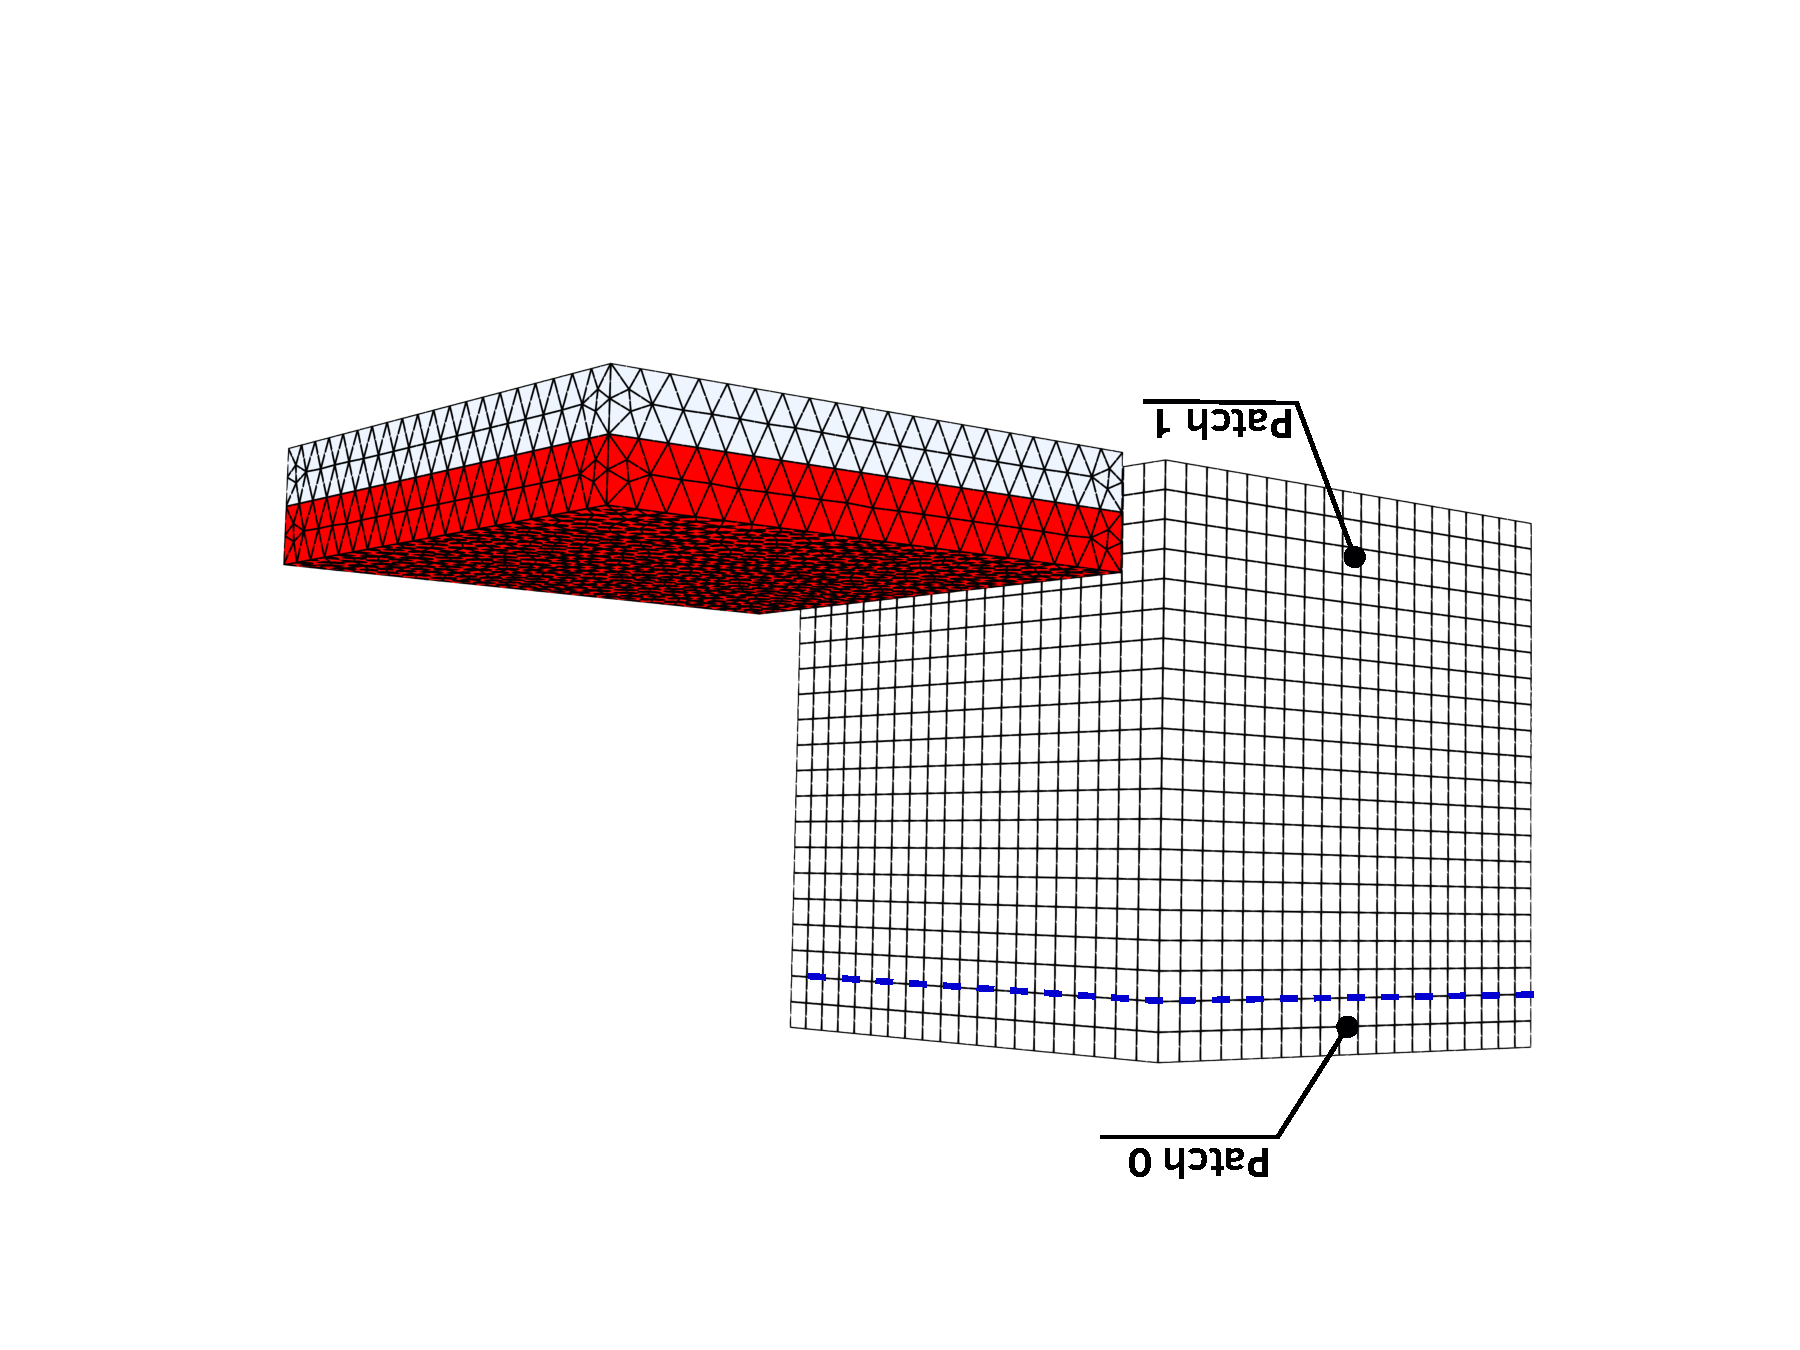
\includegraphics[trim=2cm 0.3cm 0.5cm 0cm ,clip=true,scale=1.2]{Imagens/Cap7/cavFF3d_malha.pdf}} \ 
	\subfloat[Malha do Monomodelo \label{fig:cavFF3d_malha_mono.pdf}]{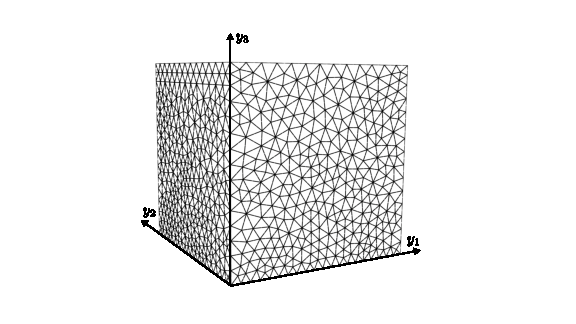
\includegraphics[scale=1.2,trim=2cm 0cm 2cm 0cm, clip=true]{Imagens/Cap7/cavFF3d_malha_mono.pdf}} \\
	\subfloat[Malha da placa \label{fig:cavFF3d_malhaPlaca}]{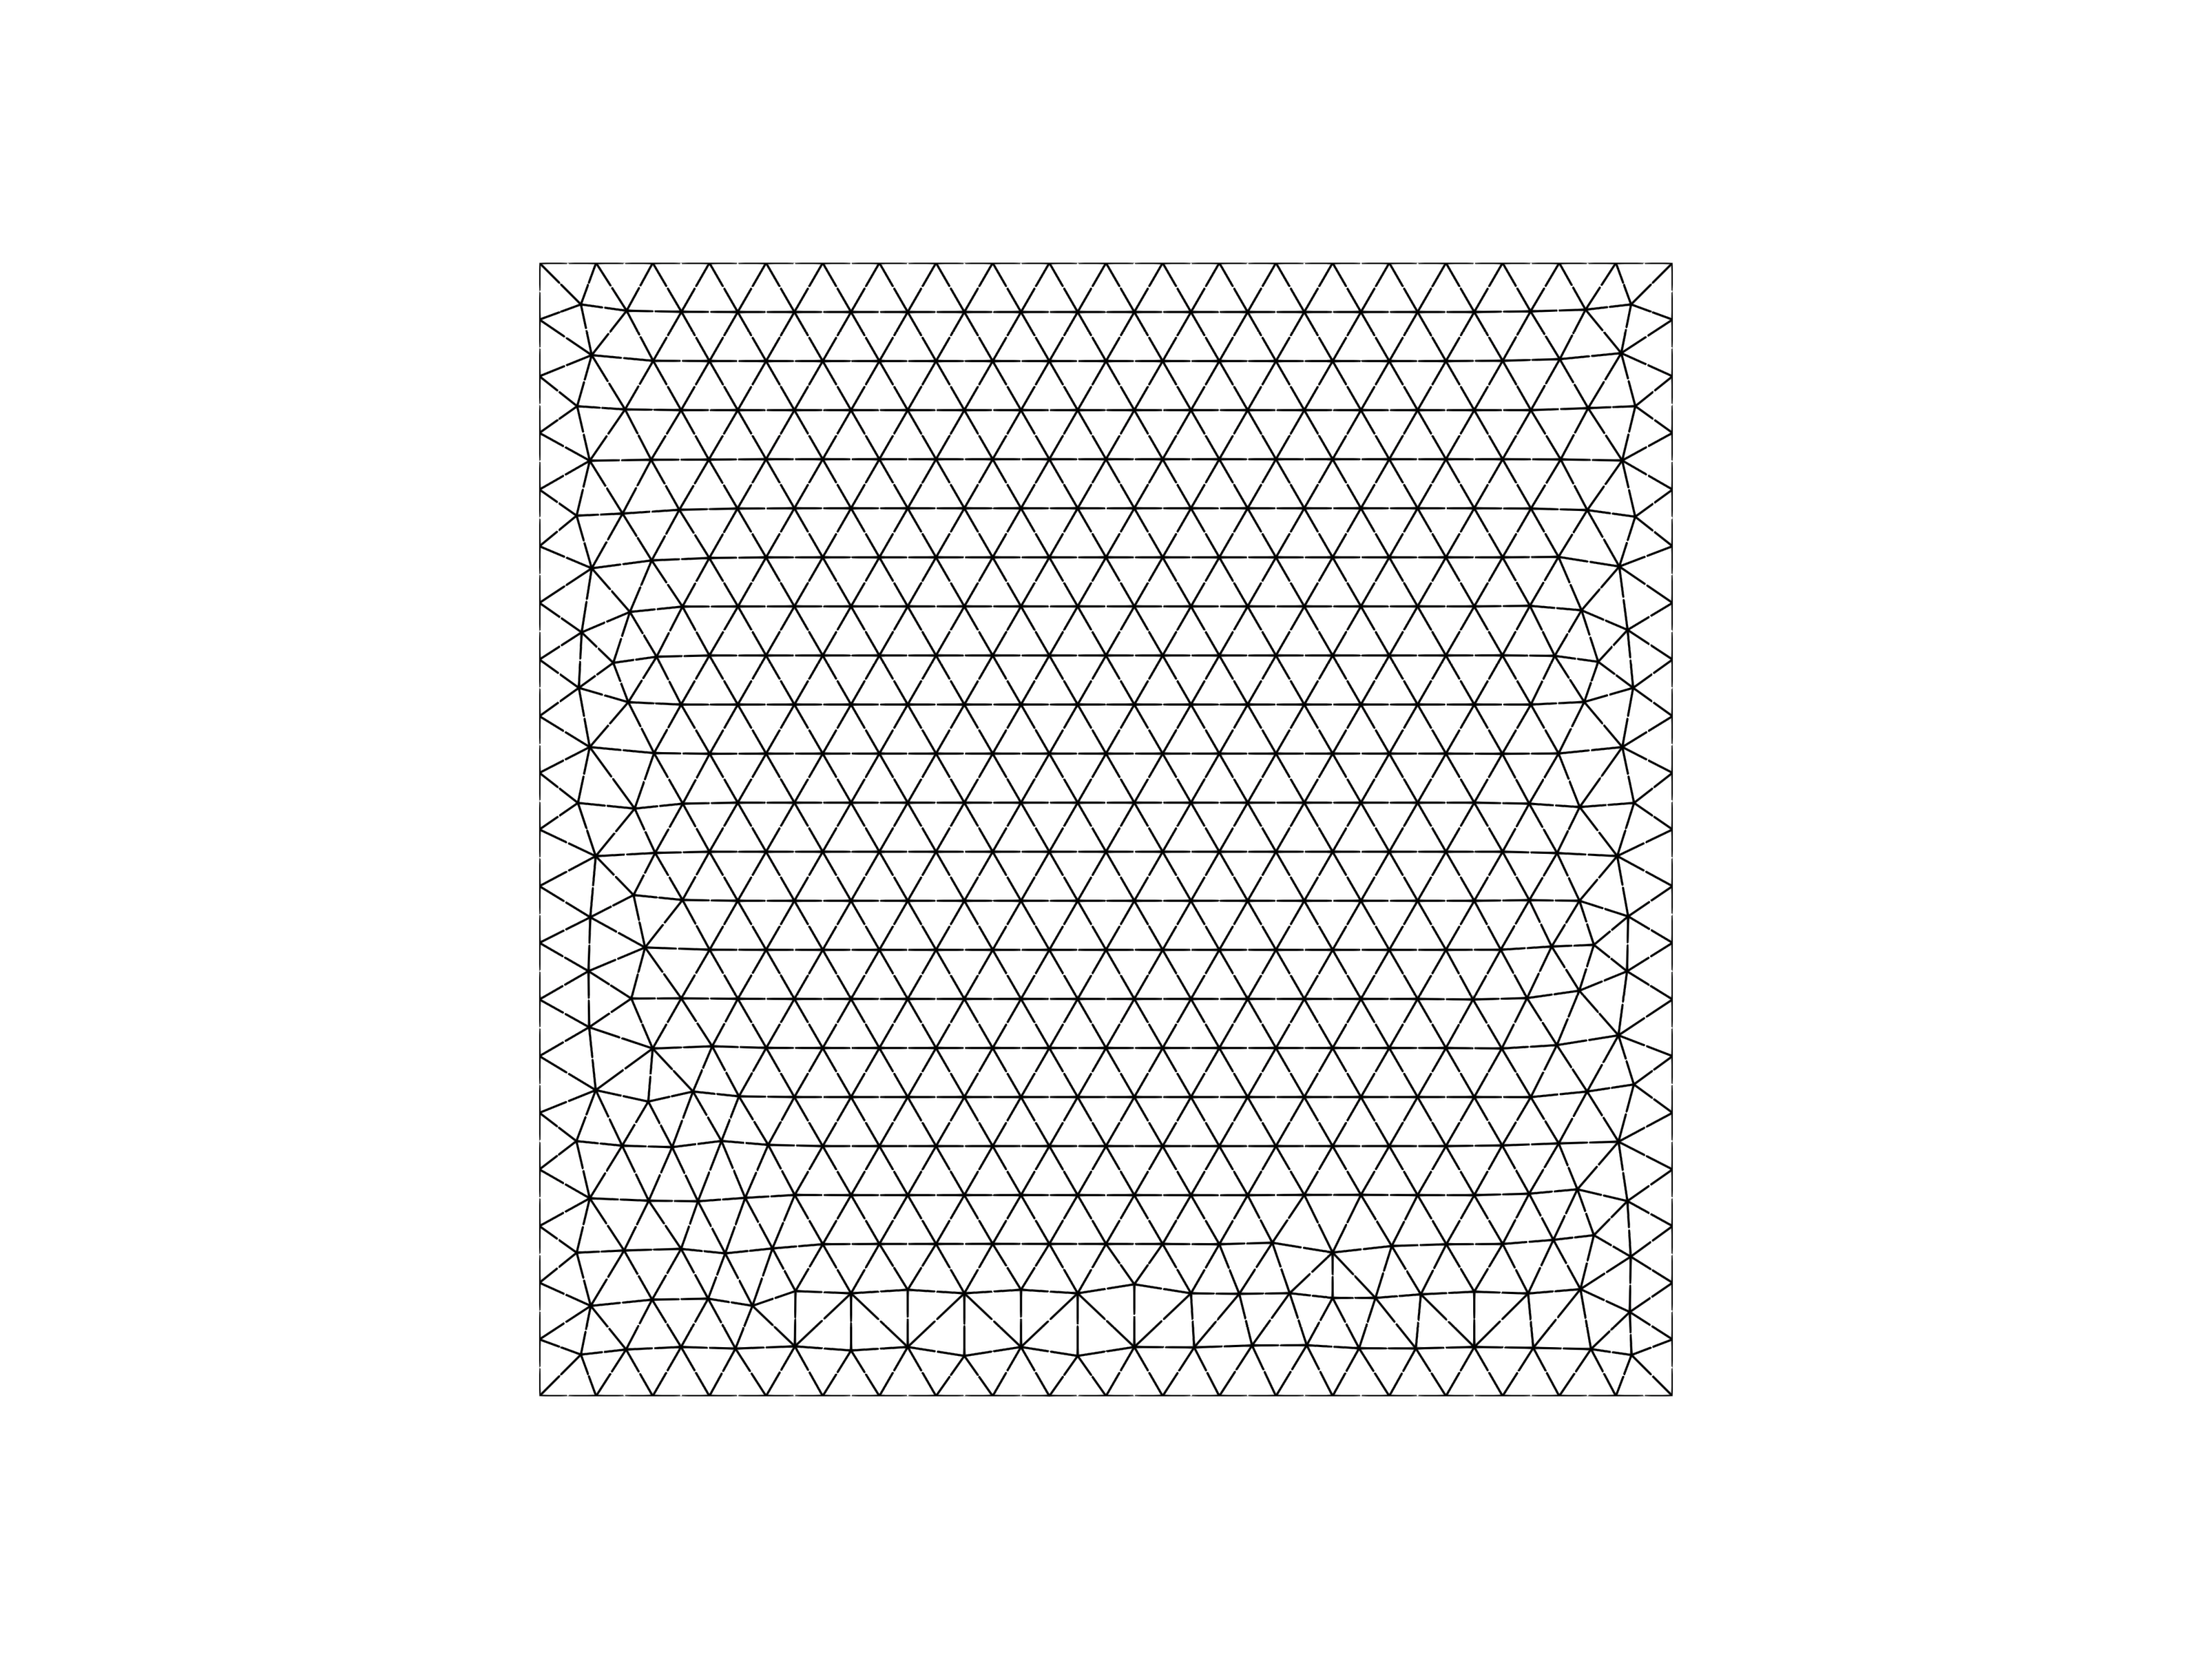
\includegraphics[scale=0.18,trim=2cm 4cm 0cm 4cm, clip=true]{Imagens/Cap7/cavFF3d_malhaPlaca.pdf}} 
	\legend{Fonte: Elaborada pela autora}
\end{figure}

O modelo Arlequin é composto por uma malha global discretizada com 2 \textit{patches} que totalizam 8000 células e 11616 pontos de controle. A malha local possui 9600 elementos e 15129 nós. A zona de colagem (ver área vermelha da Figura \ref{fig:cavFF3d_malha}) é composta por 4800 elementos e 8405 nós.  O monomodelo foi discretizado com 15895 elementos e 25127 nós. A malha da placa é constituída por 1969 nós e 944 elementos.

Na \autoref{fig:cavFF3d_deslA} pode se observar o deslocamento no ponto A que fica no centro da placa flexível para os modelos Arlequin e monomodelo, assim como os resultados dos trabalhos de \citeonline{Mok:2001},\citeonline{Vazquez:2007} e \citeonline{Yokomizo:2024}. As diferenças encontradas entre a amplitude dos deslocamentos obtidos nesse trabalho com as referências podem ser atribuídas para as diferentes formulações e discretizações adotadas para a modelagem do fluido e da chapa.

\begin{figure}[!htbp]
	\caption{Cavidade fundo flexível 3D: Deslocamento em A}
	\centering 
	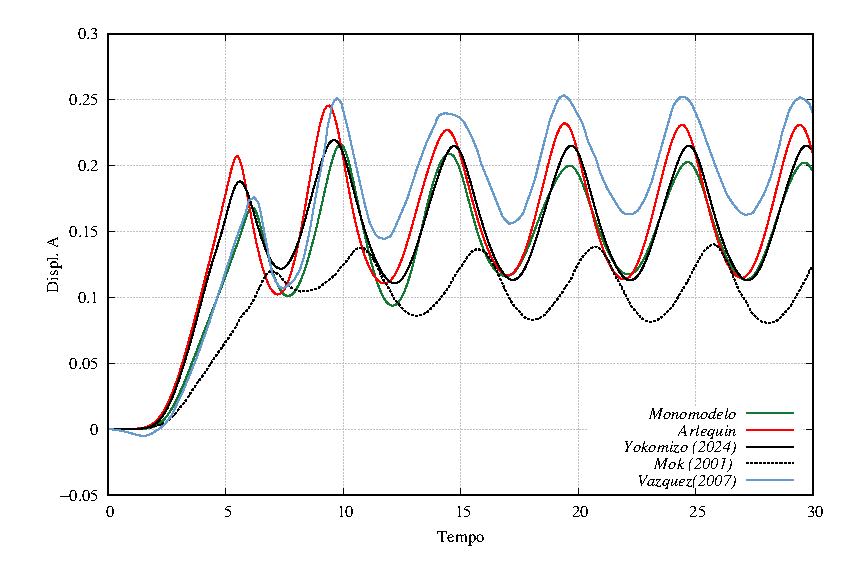
\includegraphics[scale=1.0,trim=0cm 0cm 0cm 0cm, clip=true]{Imagens/Cap7/cavFF3d_deslA.eps}	
	\label{fig:cavFF3d_deslA}
	\legend{Fonte: Elaborada pela autora}
\end{figure}

Na Figura \ref{fig:cavFF3d_vel} apresenta-se os campos de velocidade em diferentes instantes de tempo da análise; na Figura \ref{fig:cavFF3d_press}, para esses mesmos instantes, apresenta-se os campos de pressão. Por fim, na Figura \ref{fig:casca_campo_desloc} podem ser visualizados os deslocamentos na placa.

\begin{figure}[!htbp]
	\caption{Cavidade fundo flexível 3D: Campos de velocidade}
	\centering
	\subfloat[$t = 4,0 $]{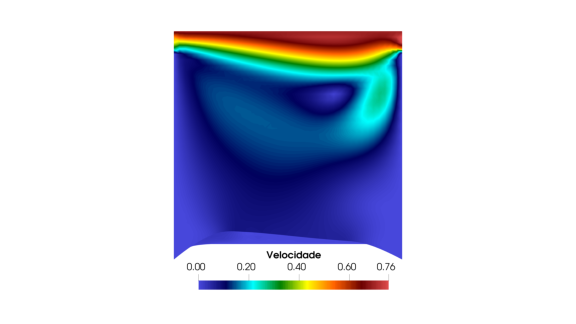
\includegraphics[scale=1.2,trim=2cm 0.3cm 2cm 0.3cm, clip=true]{Imagens/Cap7/cavFF3d_vel4.pdf}} \
	\subfloat[$t = 8,0 $]{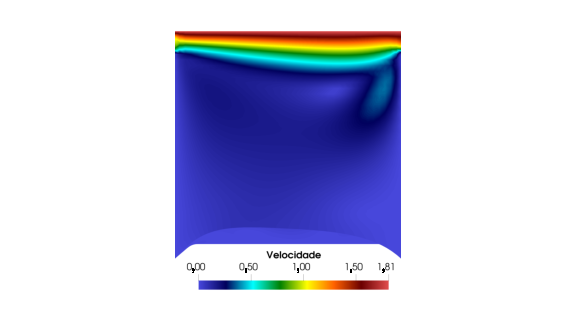
\includegraphics[scale=1.2,trim=2cm 0.3cm 2cm 0.3cm, clip=true]{Imagens/Cap7/cavFF3d_vel8.pdf}} \
	\subfloat[$t = 14,0 $]{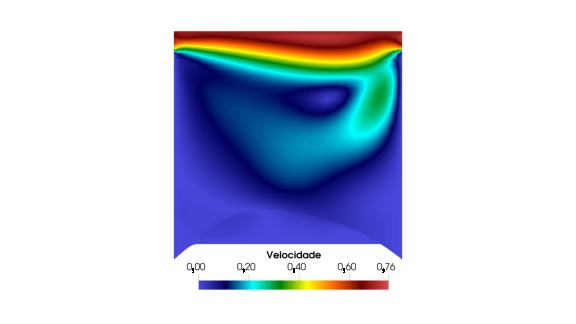
\includegraphics[scale=1.2,trim=2cm 0.3cm 2cm 0.3cm, clip=true]{Imagens/Cap7/cavFF3d_vel14.pdf}} \
	\subfloat[$t = 21,0 $]{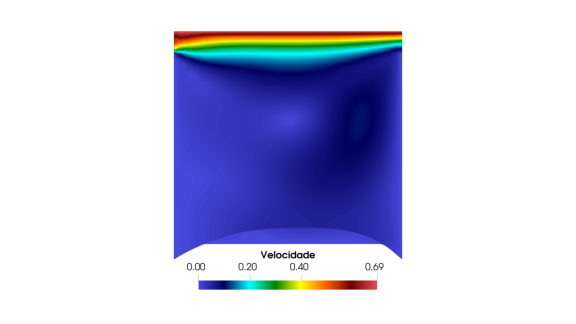
\includegraphics[trim=2cm 0.3cm 2cm 0.3cm,clip=true,scale=1.2]{Imagens/Cap7/cavFF3d_vel21.pdf}}
	\label{fig:cavFF3d_vel}
	\legend{Fonte: Elaborada pela autora}
\end{figure}

\begin{figure}[!htbp]
	\caption{Cavidade fundo flexível 3D: Campos de Pressão}
	\centering
	\subfloat[$t = 4,0 $]{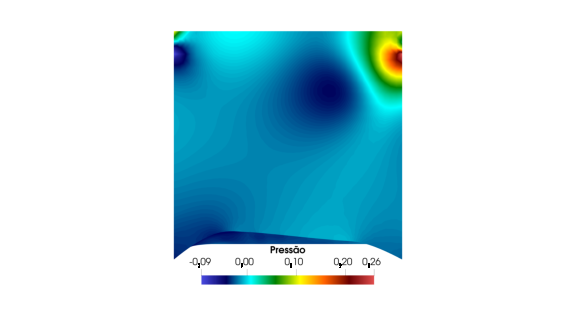
\includegraphics[scale=1.2,trim=2cm 0.3cm 2cm 0.3cm, clip=true]{Imagens/Cap7/cavFF3d_press4.pdf}} \
	\subfloat[$t = 8,0 $]{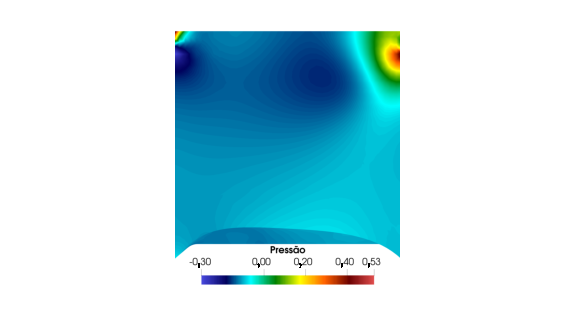
\includegraphics[scale=1.2,trim=2cm 0.3cm 2cm 0.3cm, clip=true]{Imagens/Cap7/cavFF3d_press8.pdf}} \
	\subfloat[$t = 14,0 $]{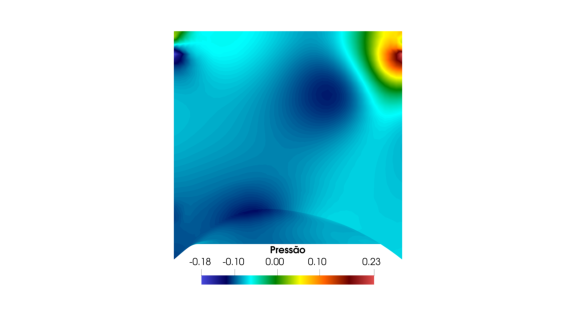
\includegraphics[scale=1.2,trim=2cm 0.3cm 2cm 0.3cm, clip=true]{Imagens/Cap7/cavFF3d_press14.pdf}} \
	\subfloat[$t = 21,0 $]{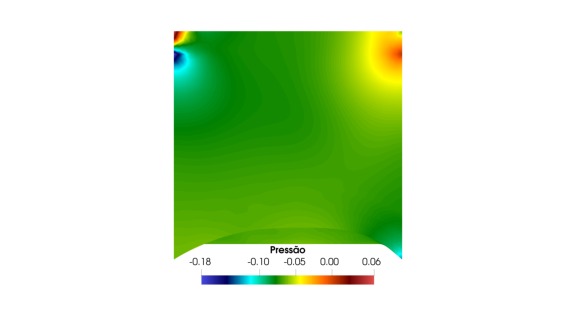
\includegraphics[trim=2cm 0.3cm 2cm 0.3cm,clip=true,scale=1.2]{Imagens/Cap7/cavFF3d_press21.pdf}}
	\label{fig:cavFF3d_press}
	\legend{Fonte: Elaborada pela autora}
\end{figure}

\begin{figure}[!htbp]
	\caption{Casca: Campos de Deslocamentos}
	\centering
	\subfloat[$t = 4,0 $]{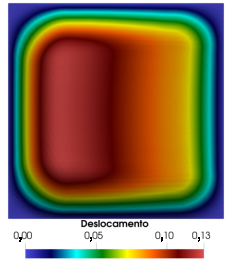
\includegraphics[scale=1.2,trim=0cm 0.0cm 0cm 0.0cm, clip=true]{Imagens/Cap7/casca_desloc_40.pdf}} \ \ \
	\subfloat[$t = 8,0 $]{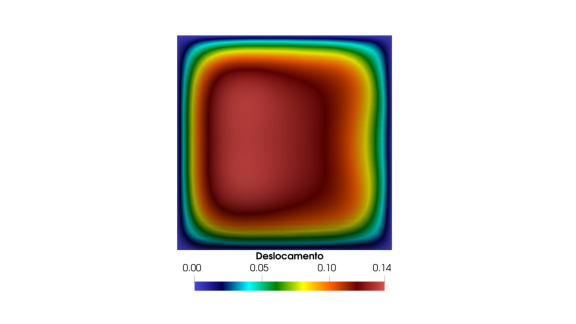
\includegraphics[scale=1.2,trim=3cm 0.5cm 3cm 0.3cm, clip=true]{Imagens/Cap7/casca_desloc_80.pdf}} \\
	\subfloat[$t = 14,0 $]{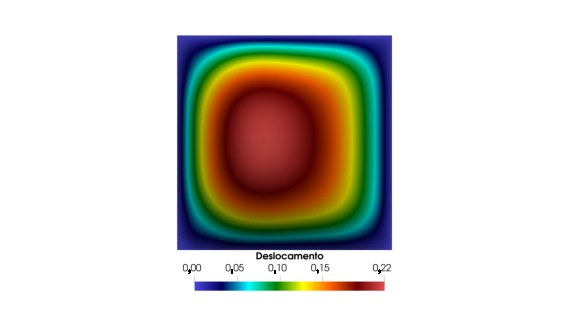
\includegraphics[scale=1.2,trim=3cm 0.3cm 3cm 0.3cm, clip=true]{Imagens/Cap7/casca_desloc_140.pdf}} \ \ \
	\subfloat[$t = 21,0 $]{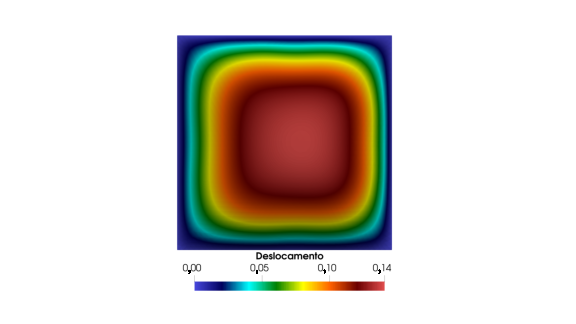
\includegraphics[trim=3cm 0.3cm 3cm 0.3cm,clip=true,scale=1.2]{Imagens/Cap7/casca_desloc_210.pdf}}
	\label{fig:casca_campo_desloc}
	\legend{Fonte: Elaborada pela autora}
\end{figure}

\subsection{\textit{Flutter} em painel flexível}

O problema dessa subseção consiste em um painel flexível engastado a um prisma rígido, conforme \autoref{fig:prisma_geometria}. Devido a complexidade dos fenômenos envolvidos nessa simulação, esse exemplo caracteriza-se por ser um dos mais utilizados na literatura para validação de formulações de IFE. Esse problema foi inicialmente proposto por \citeonline{WallR:1998}, e mais tarde, reformulado por \citeonline{Hubneretal:2004}. Essa segunda versão apresenta a mesma geometria da original, entretanto, possui alteração na velocidade de entrada e nas propriedades elásticas da estrutura. A versão apresentada por \citeonline{Hubneretal:2004}, será utilizada nesse estudo, e distingue-se por ser menos propícia a instabilidades decorrentes de acoplamento fraco. Esse problema apresenta comportamento bidimensional e aqui será simulado através de uma malha 3D utilizando-se uma profundidade de 0,1cm.

\begin{figure}[!htbp]
	\caption{Painel Flexível: Geometria}
	\centering 
	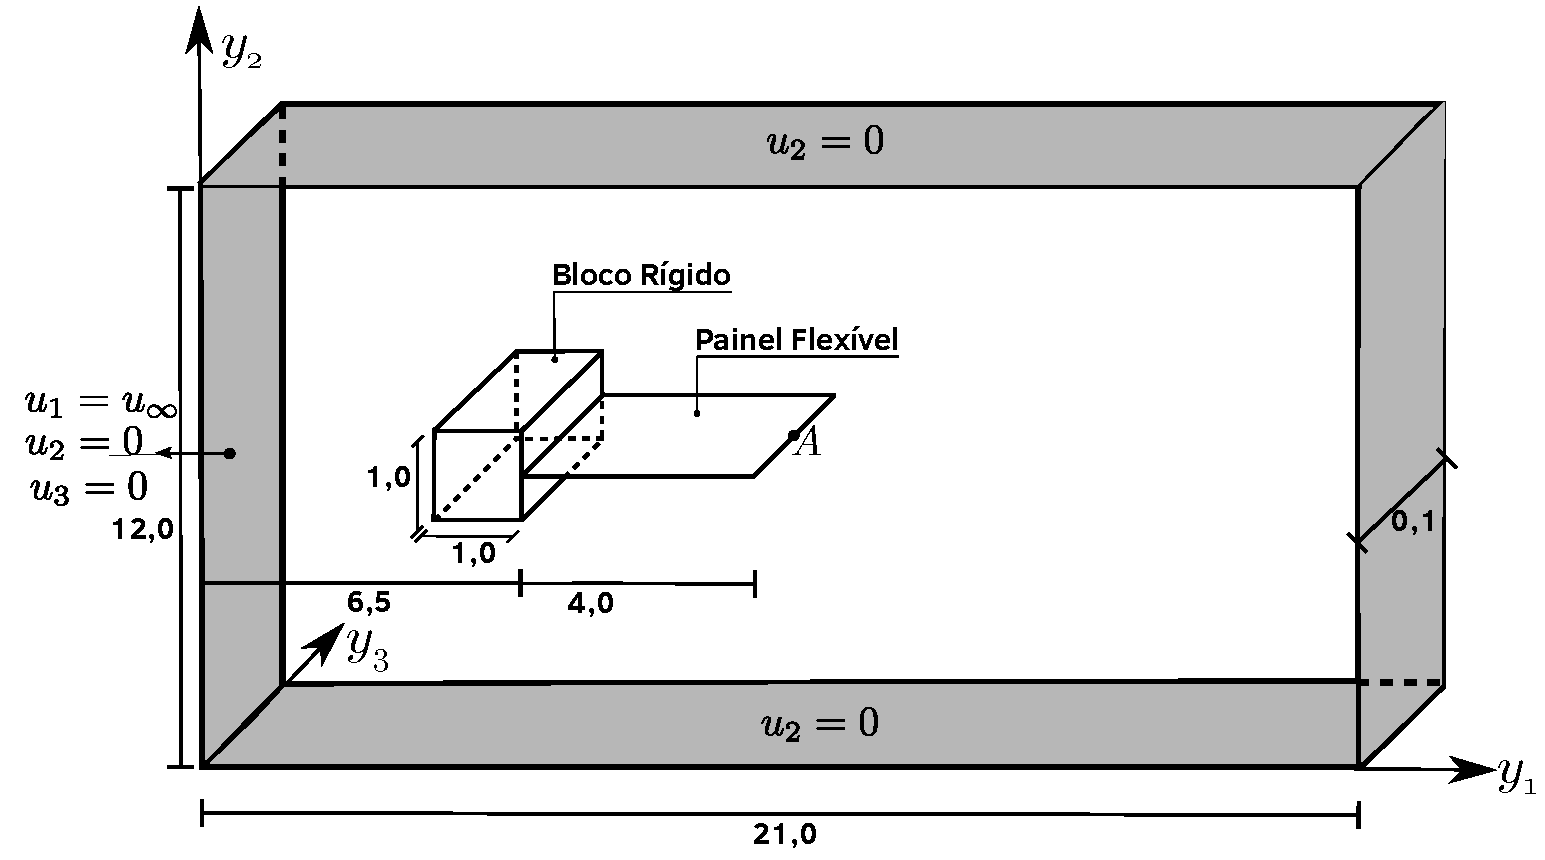
\includegraphics[scale=0.5,trim=0cm 0cm 0cm 0cm, clip=true]{Imagens/Cap7/prisma_geometria.pdf}	
	\label{fig:prisma_geometria}
	\legend{Fonte: Elaborada pela autora}
\end{figure}

A velocidade de entrada do escoamento é definida por $u_{\infty} = 31,5 cm/s$ e o fluido possui propriedades físicas do ar: viscosidade dinâmica de $\viscosity=1,82\times10^{-4} g/(cm.s)$ e massa específica equivalente a $\rho_{f} = 1,18\times10^{-3} g/cm^3 $. Tomando-se por referência o comprimento do prisma obtém-se um número de Reynolds $\Reynolds = 204$. A placa possui espessura de 0,06cm, massa específica de $\rho_{e} =  2,0 g/cm^3 $, e módulo de elasticidade caracterizado por $E = 2,0\times10^{5} g/(cm.s^2)$. Devido ao comportamento bidimensional do problema aplica-se para a placa um coeficiente de poisson  $\nu=0,0$.

Para a simulação adotou-se para o campo de velocidade inicial em todo o domínio equivalente a $u_{\infty}$. As condições de contorno para o problema são apresentadas na \autoref{fig:prisma_geometria} (com dimensões em cm). Adicionalmente adotou-se condição de simetria para o fluido na direção $y_3$, e para estrutura, nos contornos frontal e posterior, definiu-se vetor generalizado e os deslocamentos, nesta direção, como nulos.

As simulações foram conduzidas utilizando um Modelo Arlequin (Figura \ref{fig:prisma_malha}), onde a malha global é aproximada por uma discretização isogeométrica com funções quadráticas, enquanto que para malha local foram utilizados elementos finitos tetraédricos quadráticos. Além disso, um monomodelo (Figura \ref{fig:prisma_malha_mono}) foi empregado nas análises, discretizado com elementos finitos tetraédricos quadráticos. Em ambos os modelos, a placa foi representada por elementos finitos triangulares quadráticos, conforme ilustrado na Figura \ref{fig:prisma_malhaPlaca}.

\begin{figure}[!htbp]
	\caption{Painel Flexível: Discretização}
	\centering
	\subfloat[Malhas do modelo Arlequin \label{fig:prisma_malha}]{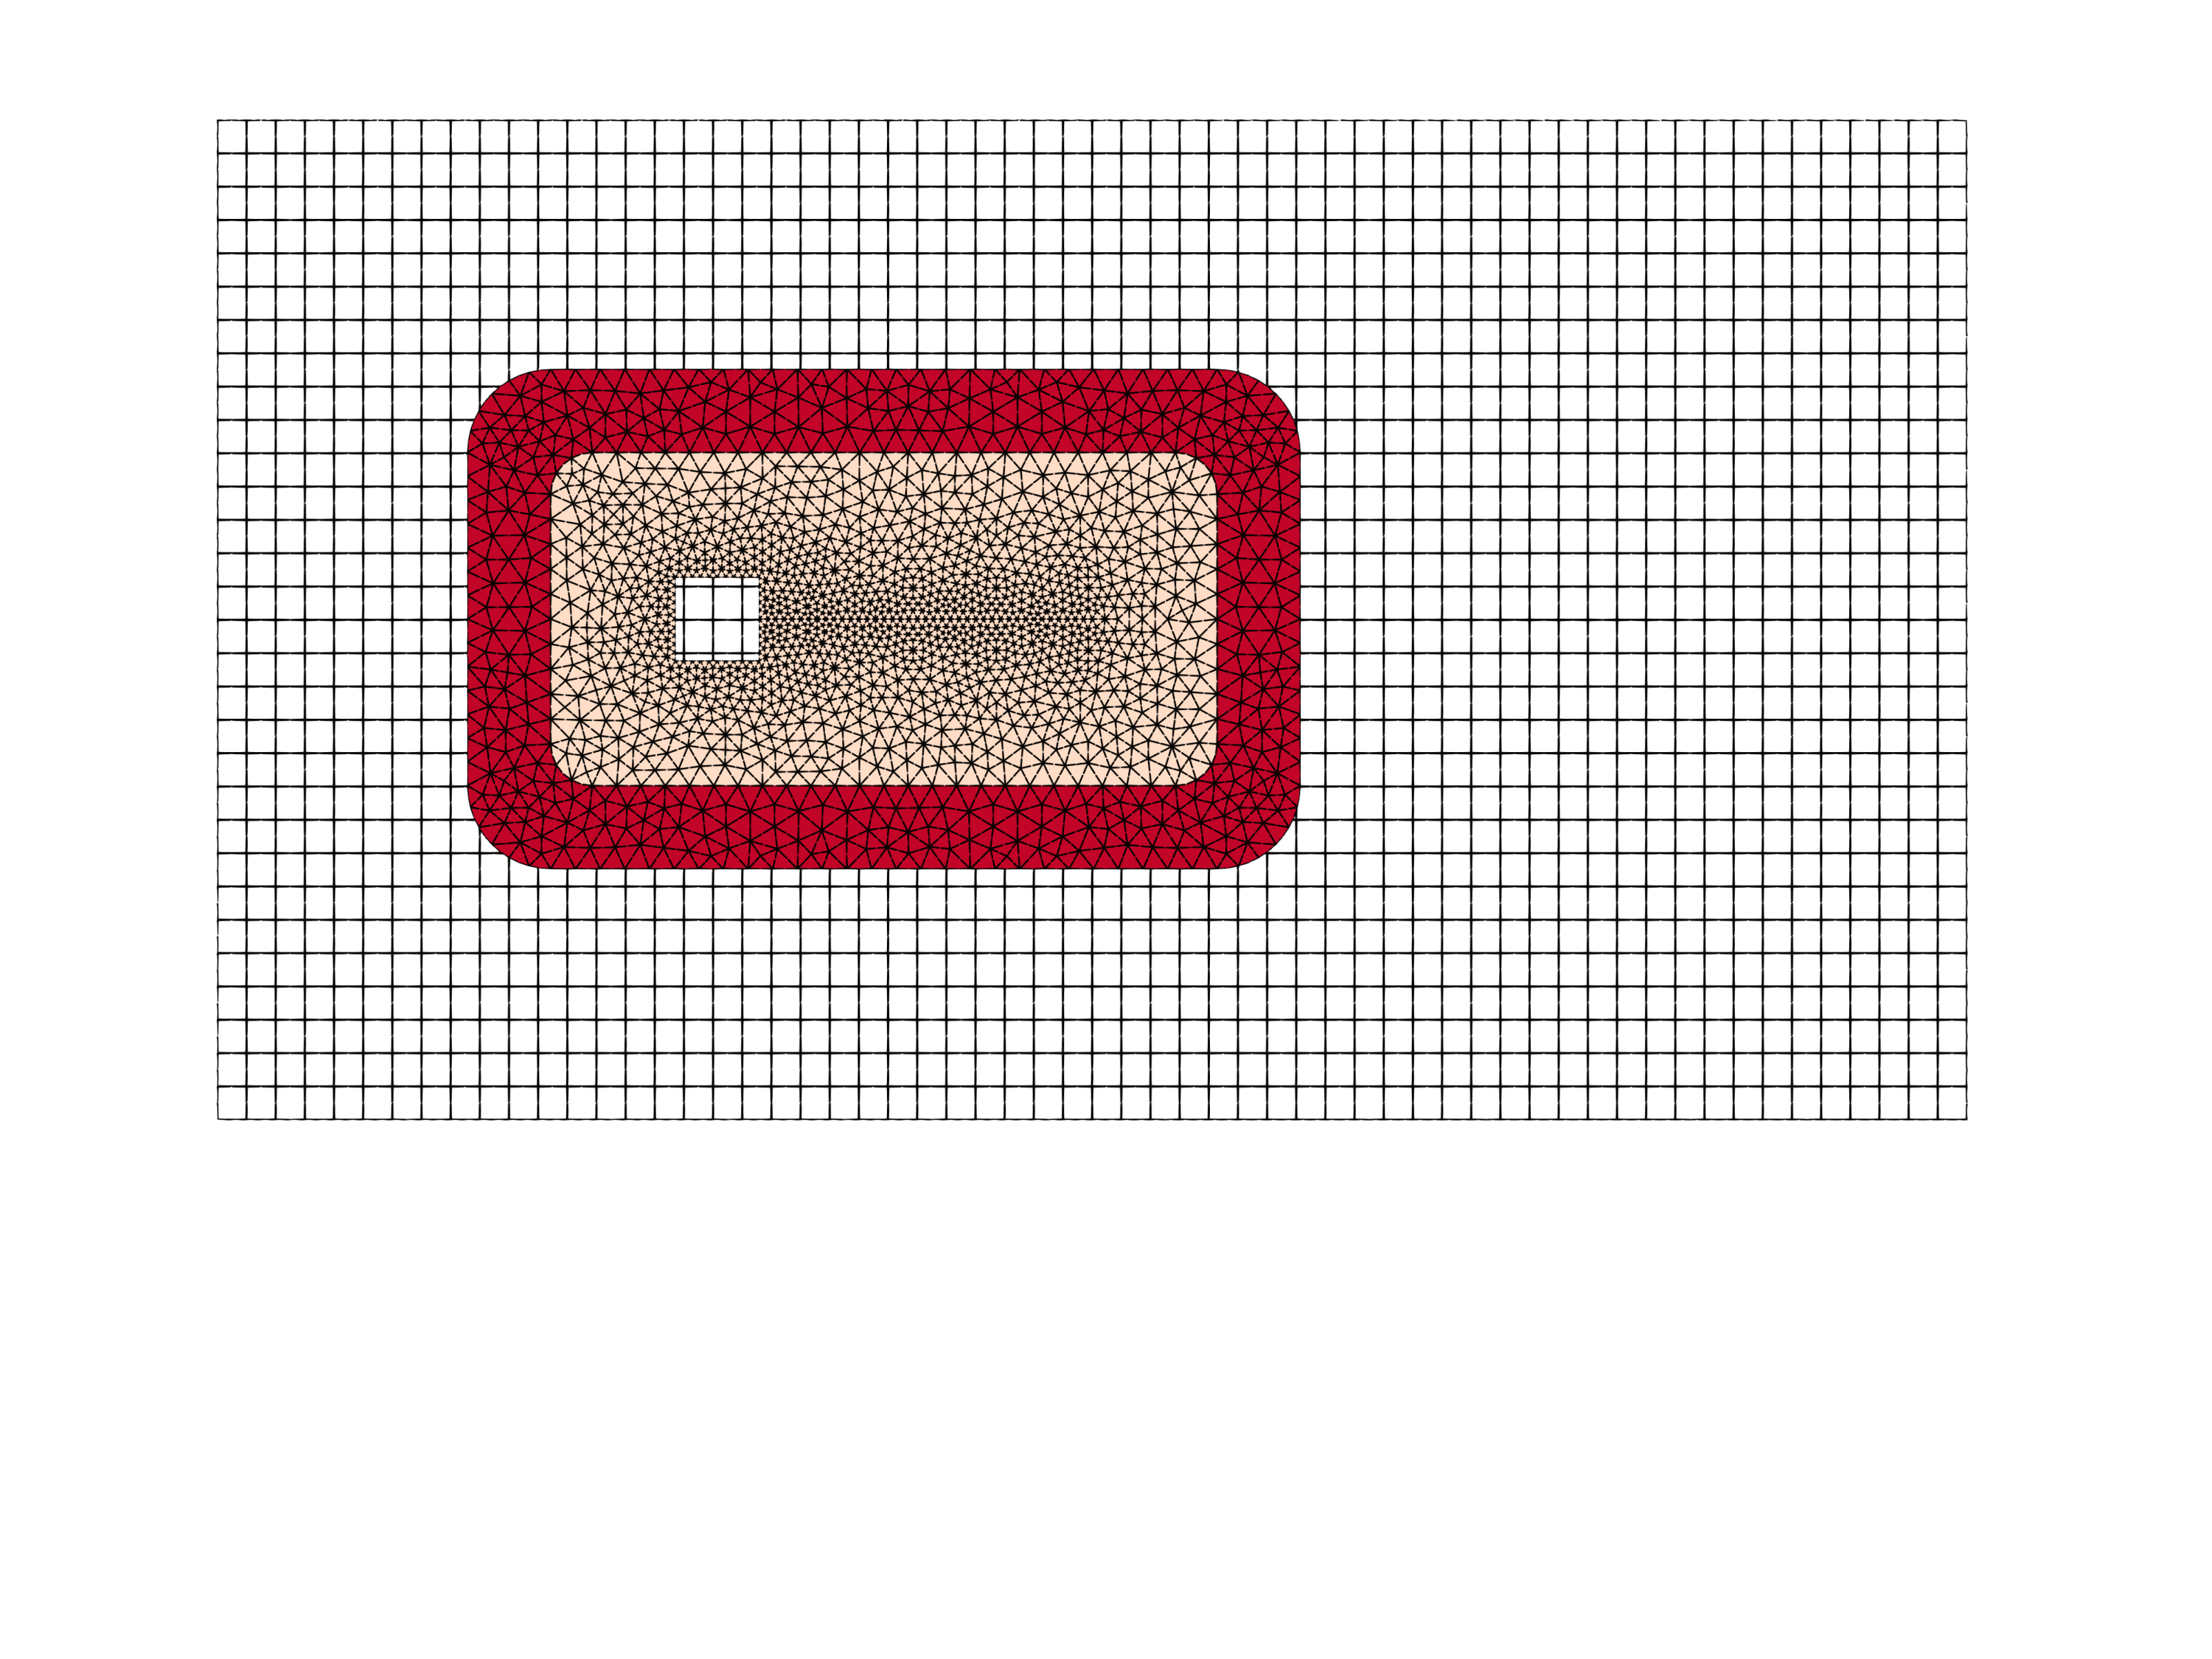
\includegraphics[scale=1.6,trim=0.5cm 1.0cm 0.5cm 0.8cm, clip=true]{Imagens/Cap7/prisma_malha.pdf}}\\
	\subfloat[Malha do monomodelo \label{fig:prisma_malha_mono}]{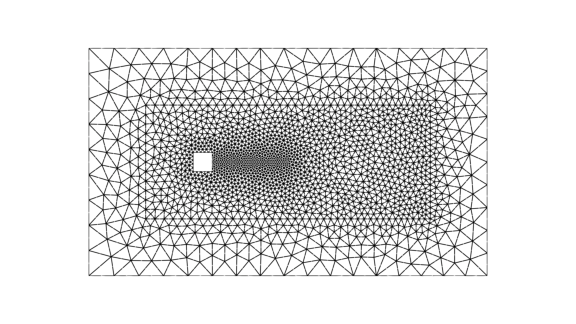
\includegraphics[scale=1.3,trim=0.5cm 0.5cm 0.5cm 0.5cm, clip=true]{Imagens/Cap7/prisma_malha_mono.pdf}}\\ 
	\subfloat[Malha da placa \label{fig:prisma_malhaPlaca}]{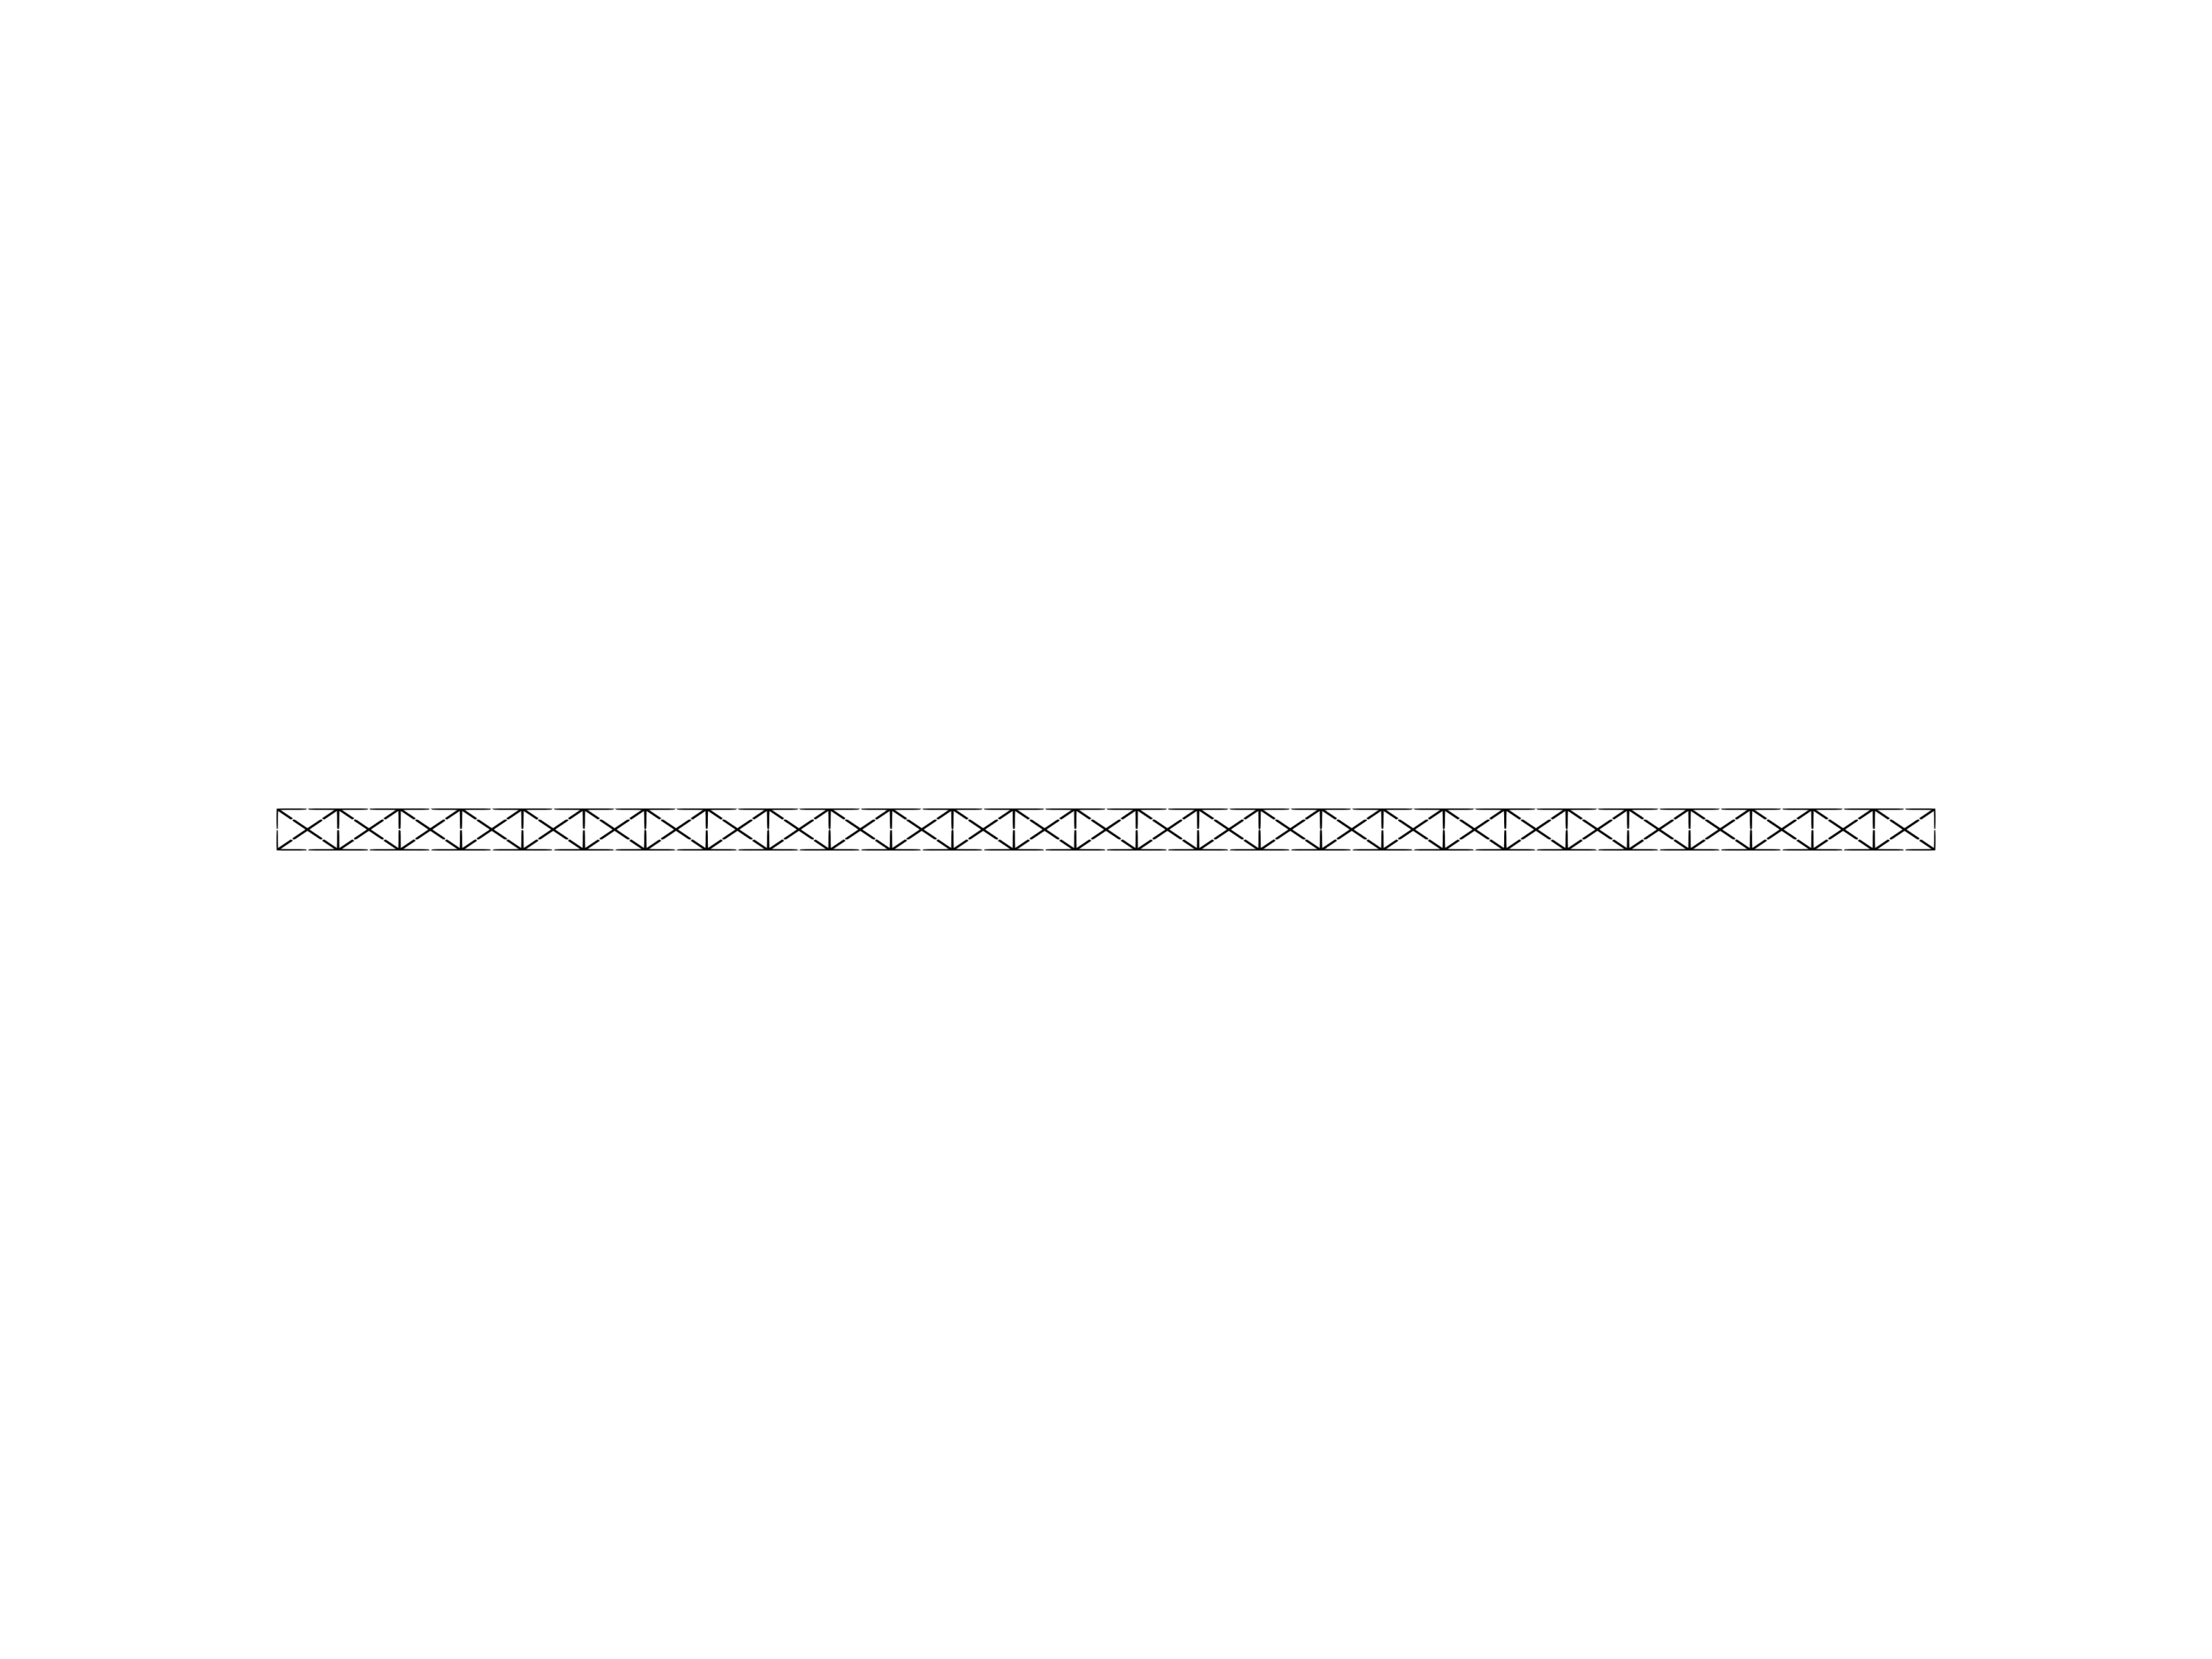
\includegraphics[scale=0.2,trim=0cm 18cm 0cm 18cm, clip=true]{Imagens/Cap7/prisma_malhaPlaca.pdf}} 
	\legend{Fonte: Elaborada pela autora}
\end{figure}

O modelo Arlequin é composto por uma malha global discretizada com 1800 elementos e 5952 pontos de controle. A malha local possui 12878 elementos e 25934 nós. A zona de colagem, com espessura de 0,2cm, de acordo com a Figura \ref{fig:prisma_malha} é composta por 1821 elementos e 4251 nós.  O monomodelo foi discretizado com 13315 elementos e 26599 nós. A malha da placa é constituída por 273 nós e 108 elementos. No que diz respeito a integração temporal utilizou-se $\timeStep = 5\times10^{-4}$, e $\specRadius = 0,5$.

\citeonline{Hubneretal:2004} obtiveram em suas simulações uma frequência de desprendimento de vórtices, considerando a placa como rígida, de $f_f = 3,7Hz$. De acordo com a teoria clássica da dinâmica das estruturas as três primeiras frequências naturais de vibração para essa estrutura de placa são $f_1 = 0,61Hz$, $f_2 = 3,80Hz$ e $f_3 = 10,63Hz$. Dessa forma, espera-se que a frequência de vibração da estrutura para o problema de IFE fique próxima a sua segunda frequência natural.

Na \autoref{fig:prisma_deslA} pode-se observar os resultados de deslocamento vertical na ponta da placa (ponto A) obtidos nesse estudo através do modelo Arlequin e do Monomodelo. Conforme pode ser observado os resultados para o monomodelo não chegam até o tempo final da análise, isto se deve em função do colapso que ocorre na malha devido aos grandes deslocamentos. Na \autoref{fig:prisma_deslA} também podem ser visualizado a envoltória dos deslocamentos obtidos por \citeonline{Hubneretal:2004}. Nota-se que os resultados desse trabalho vão se aproximando com os da referência a medida que o tempo de análise aumenta. A placa desloca-se de maneira crescente até certo ponto da análise, e a partir de então sua amplitude de vibração se mantém aproximadamente constante. 
 
\citeonline{Hubneretal:2004} obtiveram a frequência de vibração um valor de $3,1Hz$ enquanto que nesse trabalho obteve-se o valor de $3,07Hz$, calculado a partir da média dos períodos do tempo 8s até 16s. Com relação a amplitude máxima obtiveram-se valores de +0,77 e -0,77. Observa-se que a frequência de vibração da estrutura diferiu da frequência natural calculada em função dos fenômenos que ocorrem no acoplamento entre os dois meios.

\begin{figure}[!htbp]
	\caption{Painel Flexível: Deslocamento em A}
	\centering 
	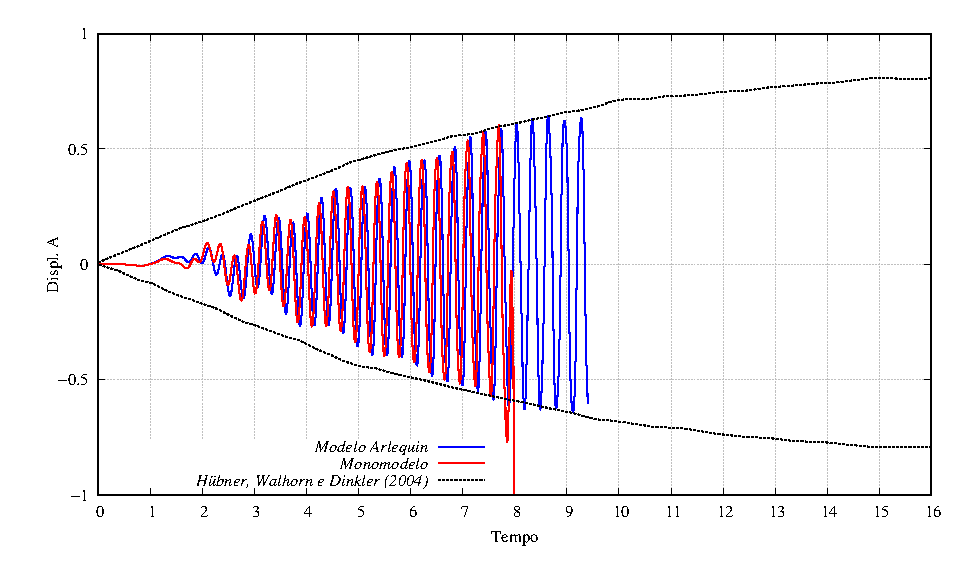
\includegraphics[scale=1.0,trim=0cm 0cm 0cm 0cm, clip=true]{Imagens/Cap7/prisma_deslA.eps}	
	\label{fig:prisma_deslA}
	\legend{Fonte: Elaborada pela autora}
\end{figure}

Considerando um ciclo de movimento da estrutura $T$ (aproximadamente periódico) apresentam-se os valores de campos de velocidade (Figura \ref{fig:prism_campos_vel} ) e de pressão (Figura \ref{fig:prism_campos_press}) para alguns instantes dentro de metade de um ciclo. Na \autoref{fig:prisma_defor_malha} apresenta-se a deformada da malha para o instante de maior deslocamento do problema.

\begin{figure}[!htbp]
	\caption{Painel Flexível: Campos de velocidade}
	\centering
	\subfloat[$nT$]{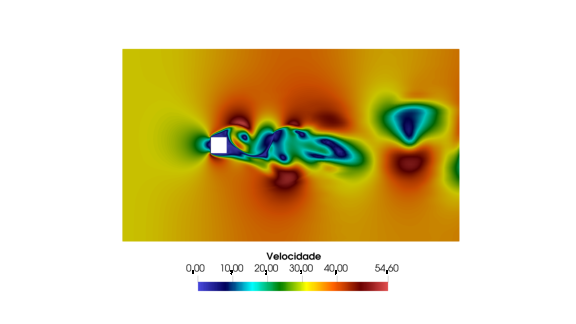
\includegraphics[scale=1.2,trim=2cm 0.5cm 2cm 0.8cm, clip=true]{Imagens/Cap7/prism_vel_19970.pdf}} \
	\subfloat[$nT + nT/12$]{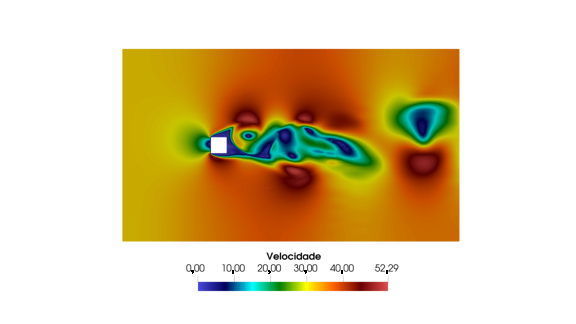
\includegraphics[scale=1.2,trim=2cm 0.5cm 2cm 0.8cm, clip=true]{Imagens/Cap7/prism_vel_20010.pdf}} \\
	\subfloat[$nT + nT/6$]{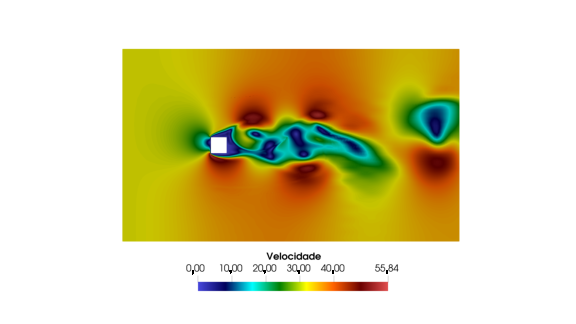
\includegraphics[scale=1.2,trim=2cm 0.5cm 2cm 0.8cm, clip=true]{Imagens/Cap7/prism_vel_20050.pdf}} \
	\subfloat[$nT + nT/4$]{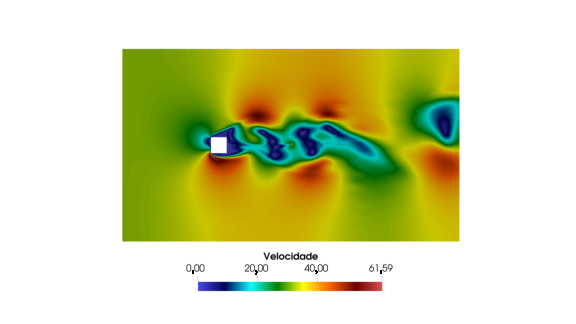
\includegraphics[scale=1.2,trim=2cm 0.5cm 2cm 0.8cm, clip=true]{Imagens/Cap7/prism_vel_20080.pdf}} \\
	\subfloat[$nT + n2T/6$]{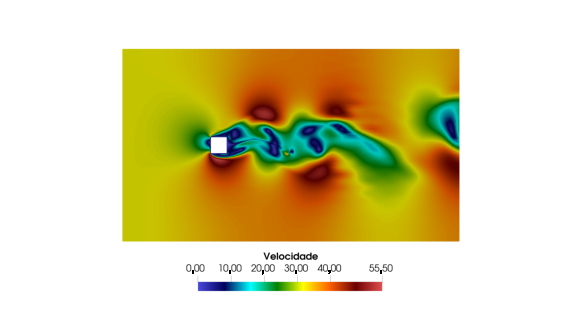
\includegraphics[scale=1.2,trim=2cm 0.5cm 2cm 0.8cm, clip=true]{Imagens/Cap7/prism_vel_20110.pdf}} \
	\subfloat[$nT + n5T/12$]{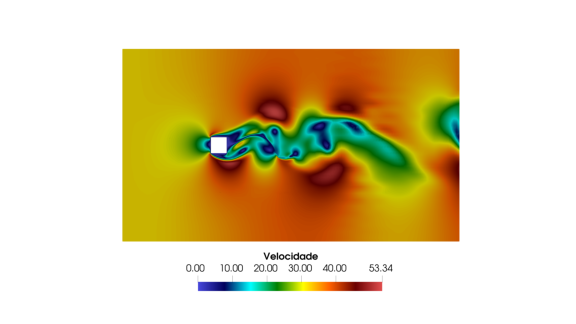
\includegraphics[scale=1.2,trim=2cm 0.5cm 2cm 0.8cm, clip=true]{Imagens/Cap7/prism_vel_20150.pdf}} \\
	\subfloat[$nT + nT/2$]{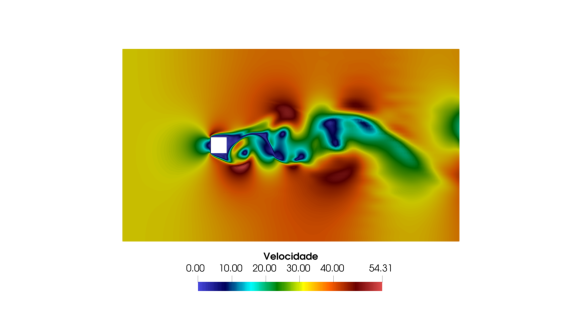
\includegraphics[scale=1.2,trim=2cm 0.5cm 2cm 0.8cm, clip=true]{Imagens/Cap7/prism_vel_20190.pdf}} 
	\label{fig:prism_campos_vel}
	\legend{Fonte: Elaborada pela autora}
\end{figure}

\begin{figure}[!htbp]
	\caption{Painel Flexível: Campos de pressão}
	\centering
	\subfloat[$nT$]{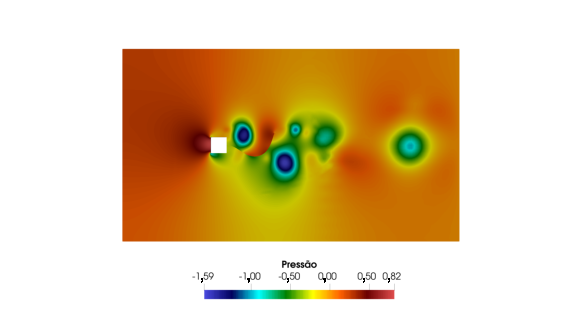
\includegraphics[scale=1.2,trim=2cm 0.4cm 2cm 0.8cm, clip=true]{Imagens/Cap7/prism_press_19970.pdf}} \
	\subfloat[$nT + nT/12$]{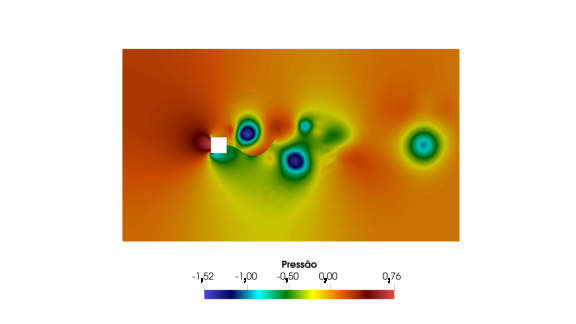
\includegraphics[scale=1.2,trim=2cm 0.4cm 2cm 0.8cm, clip=true]{Imagens/Cap7/prism_press_20010.pdf}} \\
	\subfloat[$nT + nT/6$]{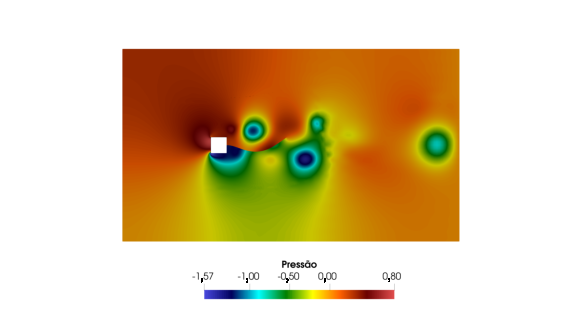
\includegraphics[scale=1.2,trim=2cm 0.4cm 2cm 0.8cm, clip=true]{Imagens/Cap7/prism_press_20050.pdf}} \
	\subfloat[$nT + nT/4$]{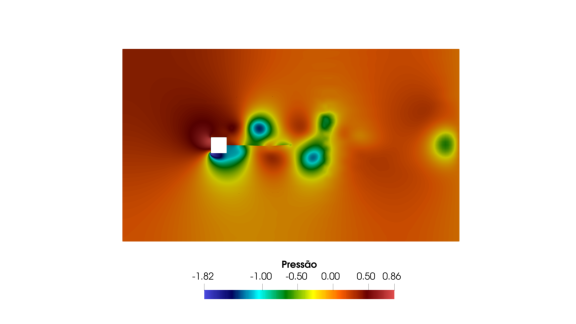
\includegraphics[scale=1.2,trim=2cm 0.4cm 2cm 0.8cm, clip=true]{Imagens/Cap7/prism_press_20080.pdf}} \\
	\subfloat[$nT + n2T/6$]{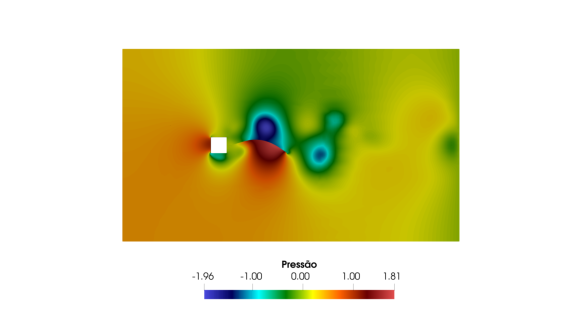
\includegraphics[scale=1.2,trim=2cm 0.4cm 2cm 0.8cm, clip=true]{Imagens/Cap7/prism_press_20110.pdf}} \
	\subfloat[$nT + n5T/12$]{\includegraphics[scale=1.2,trim=2cm 0.4cm 2cm 0.8cm, clip=true]{Imagens/Cap7/prism_press_20150.pdf}} \\
	\subfloat[$nT + nT/2$]{\includegraphics[scale=1.2,trim=2cm 0.4cm 2cm 0.8cm, clip=true]{Imagens/Cap7/prism_press_20190.pdf}}
	\label{fig:prism_campos_press}
	\legend{Fonte: Elaborada pela autora}
\end{figure}

\begin{figure}[!htbp]
	\caption{Painel Flexível: Deformada da malha em $nT$}
	\centering 
	\includegraphics[scale=1.0,trim=1cm 0.2cm 1cm 0.2cm, clip=true]{Imagens/Cap7/prism_malha_def.pdf}	
	\label{fig:prisma_defor_malha}
	\legend{Fonte: Elaborada pela autora}
\end{figure}
